%
% LaTeX report template 
%
\documentclass[a4paper,10pt]{article}
\usepackage{graphicx}
\usepackage{amsmath}
\usepackage{amssymb}
\usepackage[english]{babel}
\usepackage[latin1]{inputenc}
\usepackage[margin=1.25in]{geometry}
\graphicspath{{../img/}}

%
\begin{document}
%

   
   \title{{\large Universita' degli Studi di Padova \\ } {\normalsize Corso di laurea triennale in Ingegneria Informatica}\\ \vspace{1.8cm} \textbf{ Relazione 2\textsuperscript{a} simulazione SPICE}}

   \author{Giacomo Camposampiero, matricola 1187180}
          
   \date{24 dicembre 2020}

   \maketitle
   
   \newpage
   
   \renewcommand{\contentsname}{Indice}      
   \tableofcontents
   
   \newpage
  
\section{Esercizio primo}
Nel circuito in figura (Figure \ref{fig:ckt1}), D$_1$ e D$_2$ sono diodi ideali con una caduta di tensione in diretta V$_\gamma$=0.5 V e resistenza serie nulla. D$_3$ e' un diodo Zener con tensione di breakdown (o tensione di Zener) di 7 V, mentre la tensione di ginocchio in diretta e' V$_\gamma$=1V. V$_2$ e V$_3$ sono generatori di tensione DC V=2V, costante, mentre V$_1$ varia tra -12V e +12V.
\begin{figure}[h!]
  	\centering
 	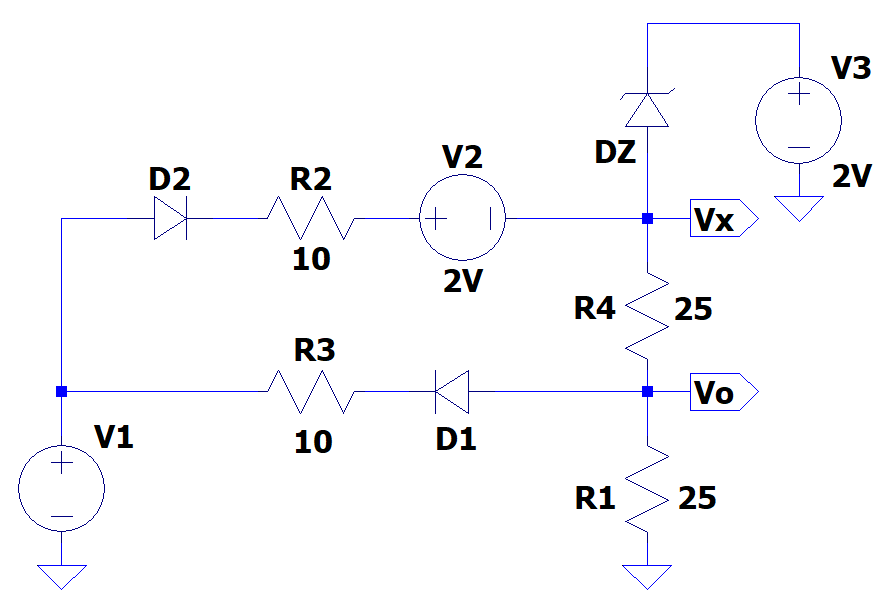
\includegraphics[width=0.6\linewidth]{ckt1.png}
  	\caption{Schema elettrico del circuito a diodi.}
  	\label{fig:ckt1}
\end{figure}

\subsection{Tracciare i grafici di V$_o$ vs V$_1$ e V$_x$ vs V$_1$ tra -12V e +12V, calcolati analiticamente}
Risolviamo analiticamente il circuito dato, studiandone una ad una tutte le diverse condizioni di funzionamento. 

\subsubsection{Ipotesi D$_1$ spento, D$_2$ spento e D$_z$ spento}
Iniziamo ipotizzando la condizione piu' semplice: D$_1$ spento, D$_2$ spento e D$_z$ spento. In questo caso i tre diodi equivalgono a tre circuiti aperti e il circuito diventa il seguente. \newline
\begin{figure}[h!]
  	\centering
 	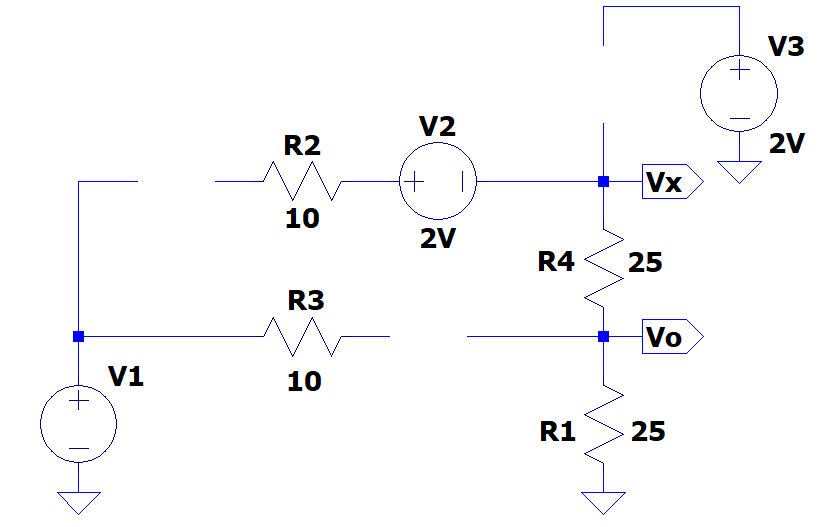
\includegraphics[width=0.3\linewidth]{es1-1-1.png}
\end{figure}

\noindent Devono quindi essere verificate le condizioni V$_{D_1}<V_{\gamma}$, V$_{D_2} < V_{\gamma}$ e $-V_{brk} < V_{D_z} < V_{\gamma}$.
Da queste possiamo derivare i vincoli equivalenti sull'ingresso variabile V$_1$
	\begin{align*}
		V_{D_1} = 0 - V_{1} < 0.5 \ \Rightarrow \ \mathbf{V_{1} >	-0.5V} \\
		V_{D_2} = V_{1} - 2V < 0.5 \ \Rightarrow \ \mathbf{V_{1} < 2.5V}
	\end{align*}
La condizione sul diodo Zener invece e' verificata per ogni valore dell'ingresso. All'interno dell'intervallo trovato nel passaggio precedente, abbiamo che \textbf{V$_o$} = \textbf{V$_x$} = \textbf{0V}. \newline

\subsubsection{Ipotesi D$_1$ spento, D$_2$ acceso e D$_z$ spento}
Lavorando in queste ipotesi, il circuito diventa il seguente. \newline
\begin{figure}[h!]
  	\centering
 	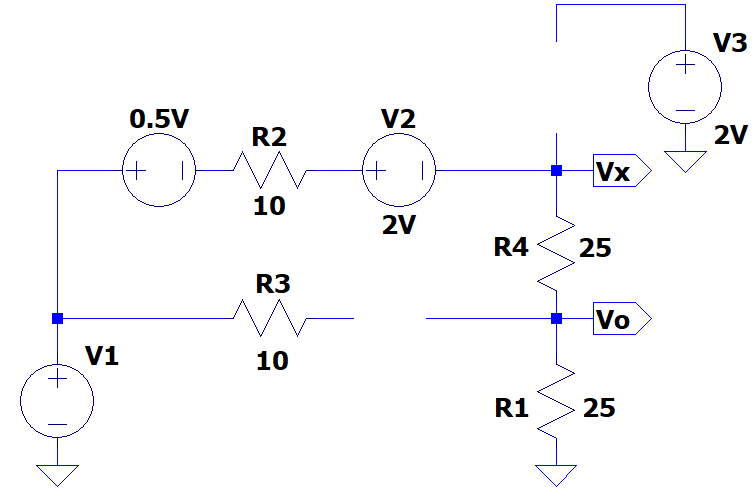
\includegraphics[width=0.3\linewidth]{es1-1-3.png}
\end{figure}

\noindent In queste ipotesi devono valere le condizioni $V_{D_1}<V_{\gamma}$, $I_{D_2}>0$ e $-7<V_{D_z}<1$. Deriviamo i conseguenti vincoli sull'ingresso variabile V$_1$ applicando le leggi di Kirchhoff delle correnti e delle tensioni, ottenendo infine
	\begin{gather*}
		I_{D_2} = \frac{V_1-2.5}{R_1+R_2+R_4}>0 \ \Rightarrow , \mathbf{V_1 > 2.5V}\\
		V_{D_1} = I_{D_2}\cdot R_1 - V_1 < 0.5 \ \Rightarrow \ V_{1} > -2.64V \\
		V_{D_z} = V_x - 2V = \frac{5V_1-24.5}{6} < 1  \ \Rightarrow \ \mathbf{V_{1} < 6.1V} \\
		V_{D_z} > -7 \ \Rightarrow \ V_{1} > -3.5V
	\end{gather*}
Nell'intervallo trovato nel passaggio precedente si hanno
	\begin{gather*}
		V_o = \frac{5}{12}(V_1 - 2.5) \\
		V_x = \frac{5}{6} (V_1 - 2.5)
	\end{gather*}

\subsubsection{Ipotesi D$_1$ spento, D$_2$ acceso e D$_z$ acceso}
Ipotizzando D$_1$ spento, D$_2$ acceso e D$_z$ acceso il circuito diventa il seguente. \newline
\begin{figure}[h!]
  	\centering
 	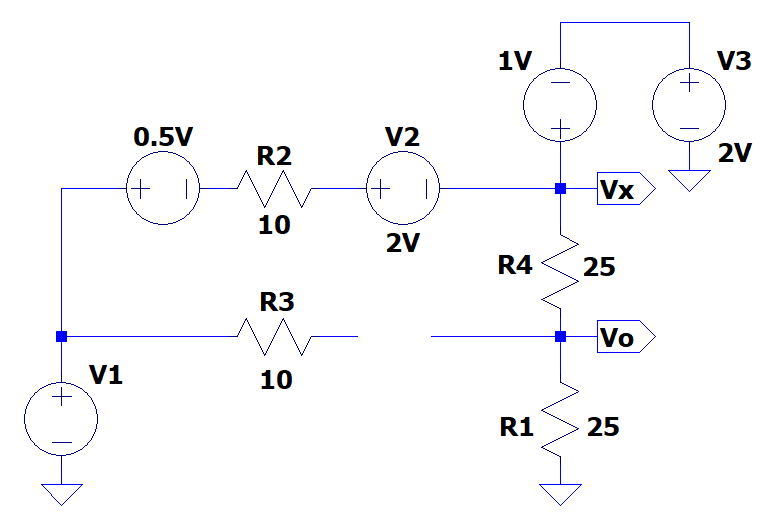
\includegraphics[width=0.3\linewidth]{es1-1-2.png}
\end{figure}

\noindent In queste ipotesi di funzionamento devono valere le condizioni $V_{D_1} < V_{\gamma}$, $I_{D_2} > 0$ e $I_{D_z} > 0$ (\textit{dove I$_{D_z}$ e' la corrente che scorre nel diodo Zener polarizzato in diretta}).
Deriviamo i conseguenti vincoli sull'ingresso variabile V$_1$ applicando le leggi di Kirchhoff delle correnti e delle tensioni, ottenendo infine
	\begin{gather*}
		I_{D_2} = \frac{V_1 - 5.5}{R_2} > 0 \ \Rightarrow \ V_{1} > 5.5V \\
		V_{D_1} = 1.5V - V_1 < 0.5 \ \Rightarrow \ V_{1} > 1V \\
		I_{D_z} = I_{D_2} - 60mA > 0 \ \Rightarrow \ I_{D_2} = \frac{V_1 - 5.5}{10} > 0.06 \ \Rightarrow \ \mathbf{V_1 > 6.1V}
	\end{gather*}
Nell'intervallo trovato nel passaggio precedente si hanno V$_x$ e V$_o$ costanti e uguali rispettivamente a 3V e 1.5V.
	
\newpage

\subsubsection{Ipotesi D$_1$ acceso, D$_2$ spento e D$_z$ in breakdown}
Lavorando in queste ipotesi, il circuito diventa il seguente. \newline
\begin{figure}[h!]
  	\centering
 	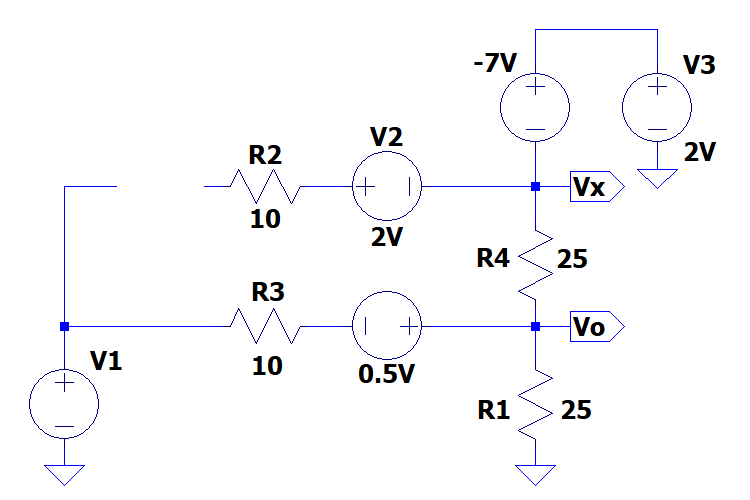
\includegraphics[width=0.3\linewidth]{es1-1-4.png}
\end{figure}

\noindent In queste ipotesi devono valere le condizioni $I_{D_1}>0$, $V_{D_2}<V_{\gamma}$ e $I_{D_z}>0$ (\textit{dove I$_{D_z}$ e' la corrente che scorre nel diodo polarizzato in inversa}). Deriviamo i conseguenti vincoli sull'ingresso variabile V$_1$ applicando le leggi di Kirchhoff delle correnti e delle tensioni, ottenendo infine
	\begin{gather*}
		V_{D_2} = V_1 + 3V < 0.5 \ \Rightarrow , V_1 < -2.5V \\
		I_{D_1} = \frac{-3 - V_1}{22.5}>0 \ \Rightarrow \ V_{1} < -3V \\
		I_{D_z} = I_{R_4} = I_{D_1}+\frac{V_o}{R_1} = \frac{-75 - 10V_1}{450} > 0 \ \Rightarrow \ \mathbf{V_1 < -7.5V}
	\end{gather*}
Nell'intervallo trovato nel passaggio precedente si hanno
	\begin{gather*}
		V_o = \frac{10V_1 - 15}{18} \\
		V_x = 5V
	\end{gather*}

\subsubsection{Ipotesi D$_1$ acceso, D$_2$ spento e D$_z$ spento}
Il circuito nelle nuove ipotesi diventa il seguente. \newline
\begin{figure}[h!]
  	\centering
 	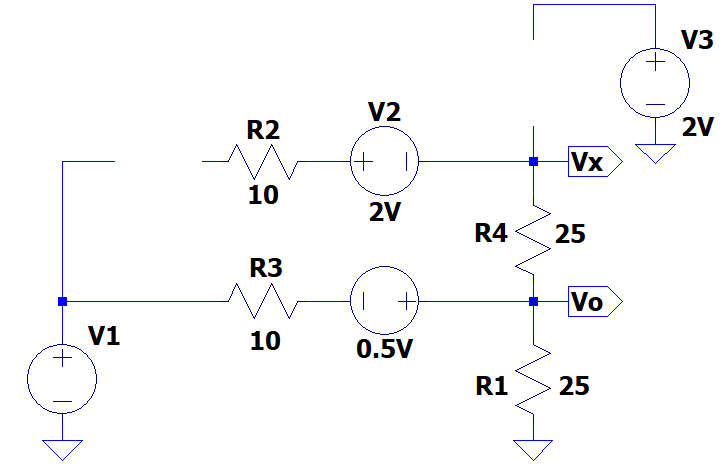
\includegraphics[width=0.3\linewidth]{es1-1-5.png}
\end{figure}

\noindent In queste ipotesi devono valere le condizioni $I_{D_1}>0$, $V_{D_2}<V_{\gamma}$ e $-7<V_{D_z}<1$. Deriviamo i conseguenti vincoli sull'ingresso variabile V$_1$ applicando le leggi di Kirchhoff delle correnti e delle tensioni, ottenendo infine
	\begin{gather*}
		I_{D_1} = \frac{-V_1 - 0.5}{R_1+R_3} > 0 \ \Rightarrow \ \mathbf{V_{1} < -0.5V} \\
		V_{D_2} = V_1 - V_x -2 = \frac{2}{7}V_1 - 2.5 < 0.5  \ \Rightarrow \ V_1 < 10.5V \\
		V_{D_z} = V_x - 2 = \frac{5V_1 - 11.5}{7} < 1  \ \Rightarrow \ V_1<3.7V \\
		V_{D_z} = \frac{5V_1 - 11.5}{7} > -7 \ \Rightarrow \ \mathbf{V_1 > -7.5V}
	\end{gather*}
Nell'intervallo trovato nel passaggio precedente si hanno
	\begin{gather*}
		V_o = V_x = \frac{5}{7}(V_1 + 0.5)
	\end{gather*}
	
Trovati i valori delle uscite in tutto l'intervallo [-12V, 12V] in cui assume valori l'ingresso V$_1$, possiamo unirne le caratteristiche ottenute nei diversi intervalli intervalli separati, ricavando infine  
	\begin{gather}
	V_o =\ \begin{cases}	\frac{5}{9}V_1 - \frac{5}{6} & \mbox{se } -7.5 < V_1 \\ 
						\frac{5}{7}V_1 + \frac{2.5}{7} & \mbox{se } -7.5 < V_1 < -0.5 \\ 
						0 & \mbox{se } -0.5 < V_1 < 2.5 \\ 
						\frac{5}{12}V_1 - \frac{12.5}{12} & \mbox{se } 2.5 < V_1 < 6.1 \\ 
						1.5 & \mbox{se } V_1>6.1 
			   \end{cases} \\ 
  	V_x =\,\begin{cases}	-5 & \mbox{se } -7.5 < V_1 \\ 
						\frac{5}{7}V_1 + \frac{2.5}{7} & \mbox{se } -7.5 < V_1 < -0.5 \\ 
						0 & \mbox{se } -0.5 < V_1 < 2.5 \\ 
						\frac{5}{6}V_1 - \frac{12.5}{6} & \mbox{se } 2.5 < V_1 < 6.1 \\ 
						3 & \mbox{se } V_1>6.1 
			   \end{cases}
	\end{gather}
I grafici V$_o$ vs V$_1$ e V$_x$ vs V$_1$ tracciati a partire dalle definizioni (1) e (2) sono riportati di seguito (rispettivamente Figure \ref{fig:graph1} e Figure \ref{fig:graph2}).

\begin{figure}[h!]
  	\centering
 	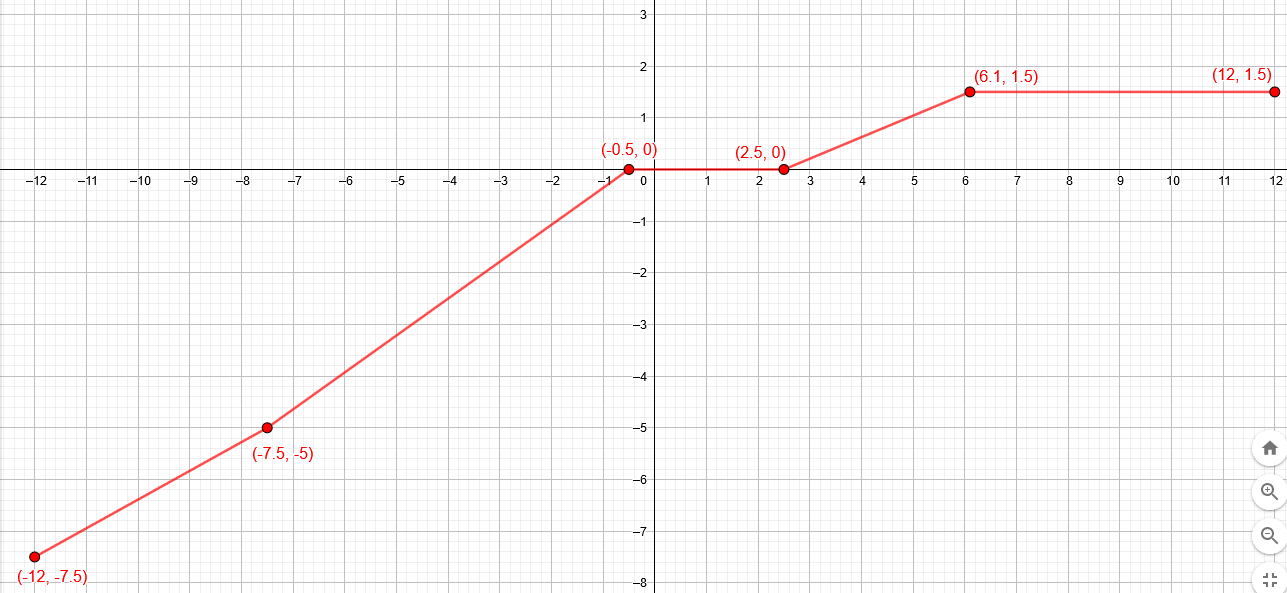
\includegraphics[width=0.9\linewidth]{es-1-1-6.png}
  	\caption{Grafico di V$_o$ in funzione di V$_1$.}
  	\label{fig:graph1}
\end{figure}

\begin{figure}[h!]
  	\centering
 	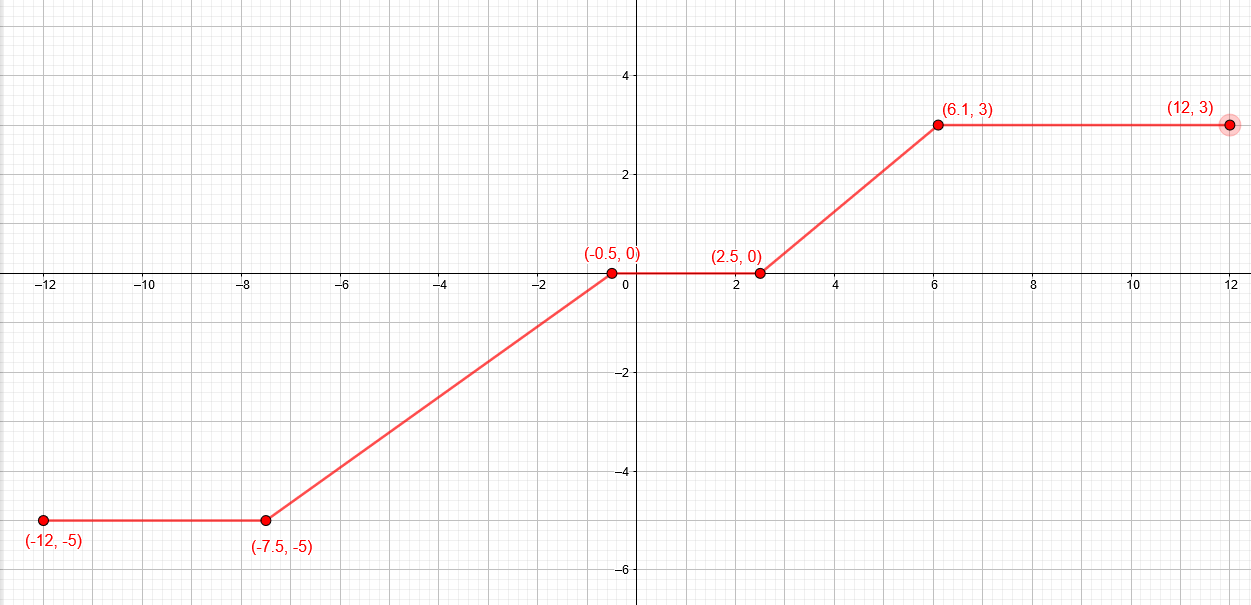
\includegraphics[width=0.9\linewidth]{es-1-1-7.png}
  	\caption{Grafico di V$_x$ in funzione di V$_1$.}
  	\label{fig:graph2}
\end{figure}

\pagebreak
\subsection{Simulare le caratteristiche V$_{out}$ vs V$_1$ e V$_x$ vs V$_1$ tra -12V e +12V con SPICE}
Il listato .cir utilizzato al fine di simulare il circuito dato e' riportato di seguito. I modelli circuitali del diodo e del diodo Zener sono quelli forniti dalla consegna. 
\begin{verbatim}
* Esercizio 1
V1 N1 0 1
* ramo diodo D2
D2 N1 N2 D
R2 N2 N3 10
V2 N3 Vx 2V
* ramo zener
V3 N5 0 2V
DZ Vx N5 DZ
* ramo diodo D1
R3 N1 N4 10
D1 Vo N4 D
* altri rami
R4 Vo Vx 25
R1 0 Vo 25
.dc V1 -12 12 0.1
.model D D RON=0 VFWD=0.5
.model DZ D VFWD=1.0V VREV=7V
.backanno
.end
\end{verbatim}

Le caratteristiche V$_{out}$ vs V$_1$ e V$_x$ vs V$_1$ tra -12V e +12V sono riportate in figura (Figure \ref{fig:spice1}) in un unico grafico. Gli intervalli in cui si vede un solo colore corrispondono agli intervalli nei quali i due segnali si sovrappongono. E' riportato anche un grafico delle correnti misurate nei diversi rami a cui appartengono i diodi, ritenuto particolarmente significativo rispetto allo studio del circuito in esame (Figure \ref{fig:dioditot}).

\begin{figure}[h!]
  	\centering
 	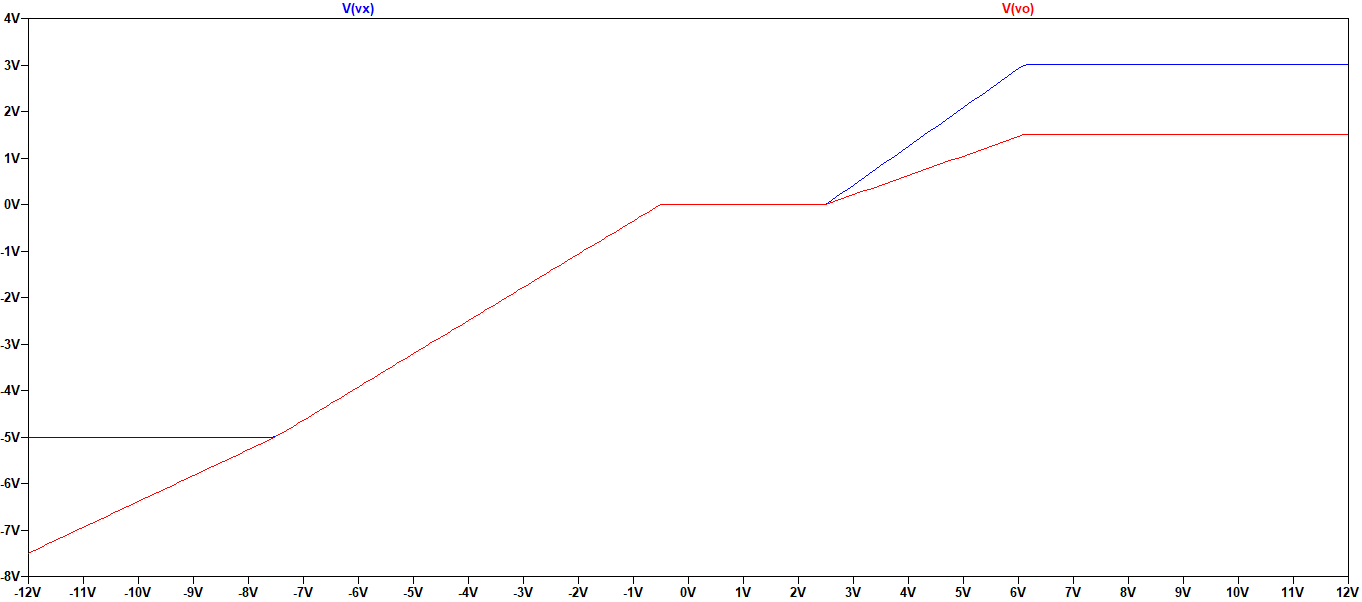
\includegraphics[width=1\linewidth]{es1-2.png}
  	\caption{Risultato della simulazione SPICE.}
  	\label{fig:spice1}
\end{figure}

\begin{figure}[h!]
  	\centering
 	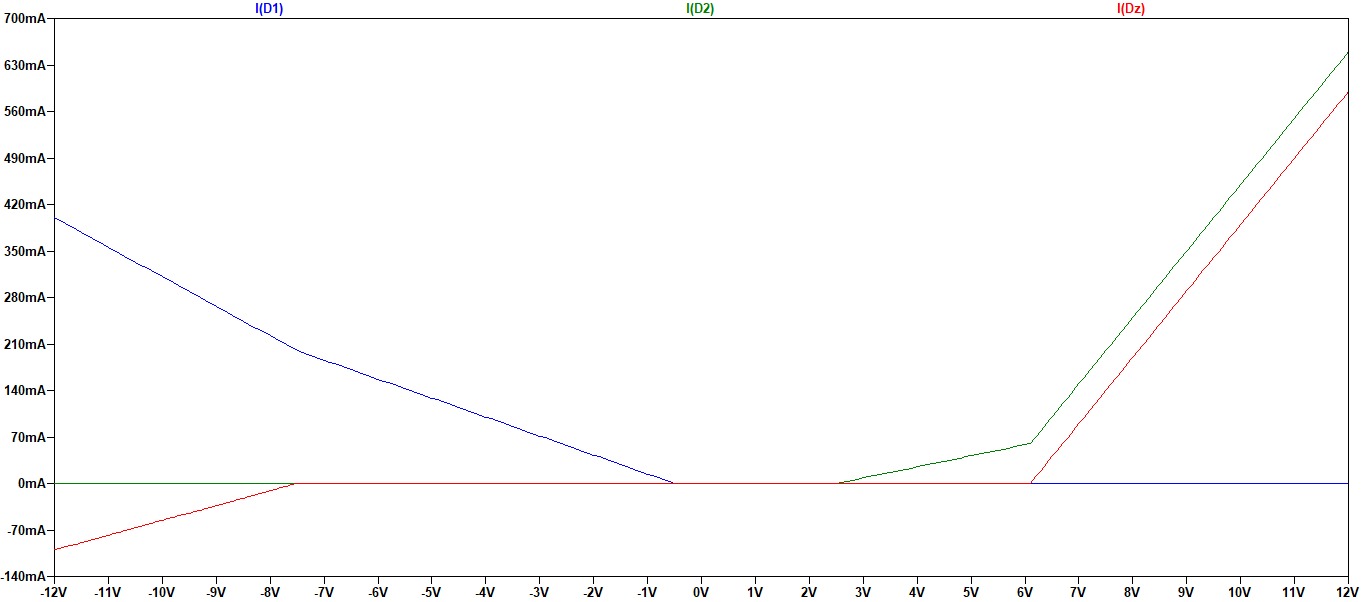
\includegraphics[width=1\linewidth]{es1-2-1.png}
  	\caption{Correnti che attraversano i tre diodi.}
  	\label{fig:dioditot}
\end{figure}

\vspace*{1cm}

\subsection{Qual e' la massima potenza dissipata dal diodo Zener?}
La massima potenza dissipata dal diodo Zener e' stata trovata per via sperimentale, graficando la potenza dissipata dal diodo e svolgendo un'analisi qualitativa dei dati ottenuti. Come si puo' notare dalla caratteristica della potenza (Figure \ref{fig:pwd1}), la massima potenza dissipata dal diodo Zener e' $700\,mW$.

\begin{figure}[h!]
  	\centering
 	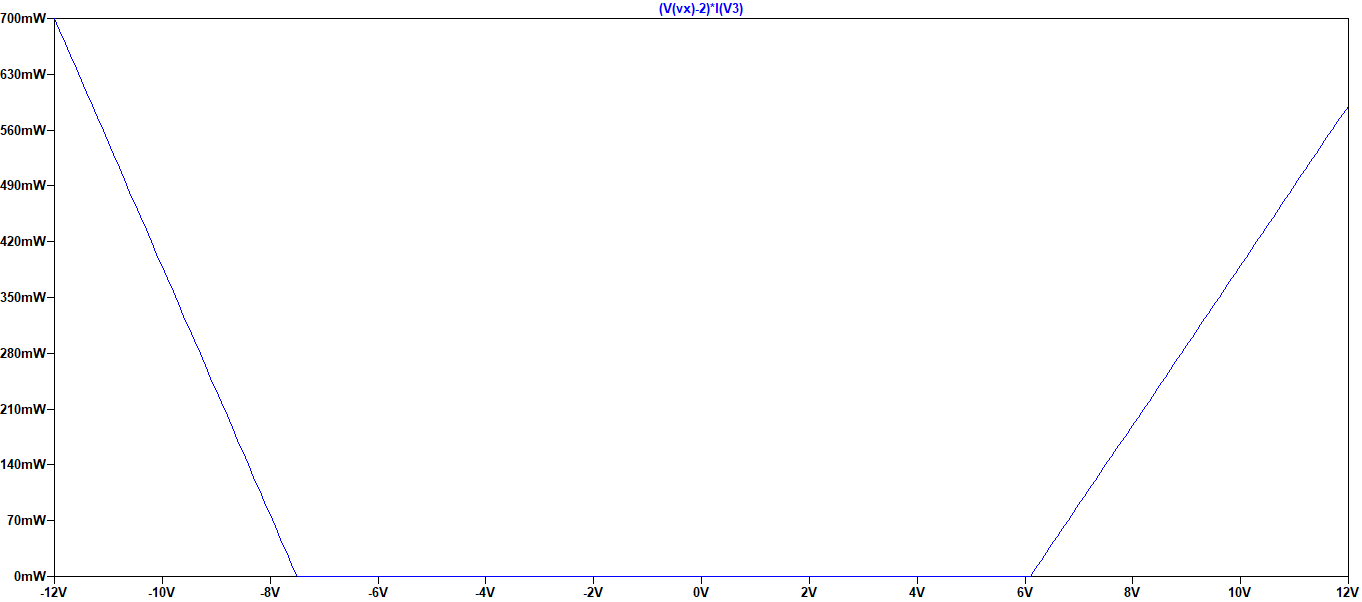
\includegraphics[width=1\linewidth]{es1-3.png}
  	\caption{Potenza dissipata dal diodo Zener.}
  	\label{fig:pwd1}
\end{figure}

\pagebreak

\section{Esercizio secondo}
Il circuito in figura (Figure \ref{fig:ckt2}) rappresenta un amplificatore a source comune con circuito di autopolarizzazione. Il transistor N-MOS ha una tensione di soglia V$_{tn}$ pari a 1V, k$^{'}_{n}$=8$\frac{mA}{V^2}$, W=100$\mu$m e L=2$\mu$m, $\lambda$=0. All'ingresso e' connesso un generatore di tensione sinusoidale di ampiezza 10
mV, frequenza 1kHz; all'uscita una resistenza di carico da 1k$\Omega$.

\begin{figure}[h!]
  	\centering
 	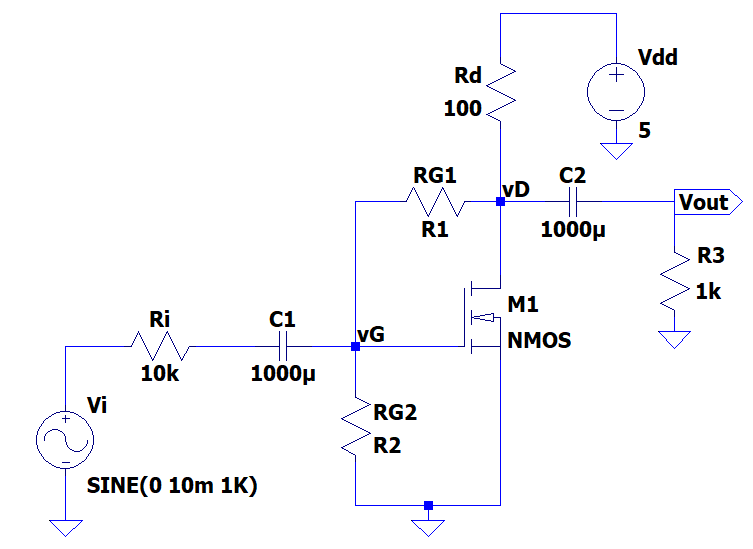
\includegraphics[width=0.6\linewidth]{ckt2.png}
  	\caption{Schema elettrico dell'amplificatore.}
  	\label{fig:ckt2}
\end{figure}

\subsection{Porre R$_{G1}$ pari al proprio numero di matricola, R$_{G2}$=$\infty$}

\subsubsection{Calcolare analiticamente il punto di polarizzazione DC del transistor}
Per prima cosa, disegniamo il circuito equivalente nell'analisi a largo segnale (Figure \ref{fig:pol1}), in cui tutti i condensatori equivalgono a circuiti aperti e tutti i segnali non DC sono annullati.

\begin{figure}[h!]
 	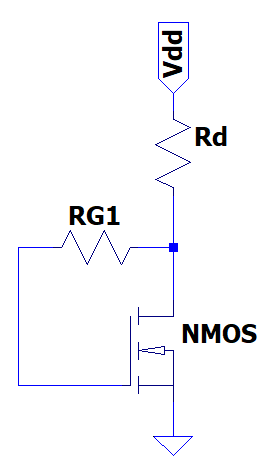
\includegraphics[width=0.16\linewidth]{pol1.png}
 	\centering
 	\caption{Circuito equivalente per largo segnale.}
  	\label{fig:pol1}
\end{figure}

Possiamo notare che $V_{DSQ}=V_{GSQ}$ (in quanto nel ramo che collega drain e gate del transistor non scorre corrente), per cui il mosfet si trova in saturazione. A questo punto, risolviamo il seguente sistema (nel quale le due equazioni derivano rispettivamente dalla relazione della corrente di drain di un N-MOS enhancement in saturazione e dalla legge di Kirchhoff delle tensioni sulla maglia V$_{DD}$-massa) nell'incognita V$GSQ$.

\begin{align*}
	\begin{cases}
		I_{DQ} = \frac{k_n}{2} \cdot (V_{GSQ}-V_{tn})^2 \\[4pt]
		I_{DQ} = \frac{V_{DD}-V_{GSQ}}{R_D}
	\end{cases}
\end{align*}

\noindent Il risultato del sistema e' un'equazione di secondo grado nell'incognita V$_{GSQ}$
\begin{align*}
0.2 V_{GSQ}^2 - 0.39 V_{GSQ} + 0.15 = 0 
\end{align*}
le cui soluzioni sono
\begin{align*}
V_{GSQ} = V_{DSQ} = 1.42V \ \Rightarrow \  V_{GSQ} - V_{tn} = \mathbf{0.42V}  \textit{  ok}\\
V_{GSQ} = V_{DSQ} = 0.53V \  \Rightarrow \ V_{GSQ} - V_{tn} = -0.47V < 0 \textit{  no}
\end{align*}
Possiamo infine calcolare la corrente di drain in polarizzazione, che equivale a 
\begin{align*}
I_{DSQ} = \frac{k_n}{2}\cdot V_{ov}^2 = 35.77 mA
\end{align*}

\subsubsection{Calcolare i parametri del il modello per piccolo segnale}
Il calcolo dei parametri del modello per piccolo segnale e' riportato di seguito
\begin{align*}
g_m = k_n \cdot V_{ov} = 168mS \qquad \qquad \qquad r_o = \infty
\end{align*}

\subsubsection{Disegnare il modello per piccolo segnale dell'amplificatore e calcolare il guadagno in tensione, R$_{in}$ e R$_o$.}
Il modello per piccolo segnale dell'amplificatore a source comune in esame e' rappresentato di seguito (Figure \ref{fig:pic1}). 
\begin{figure}[h!]
 	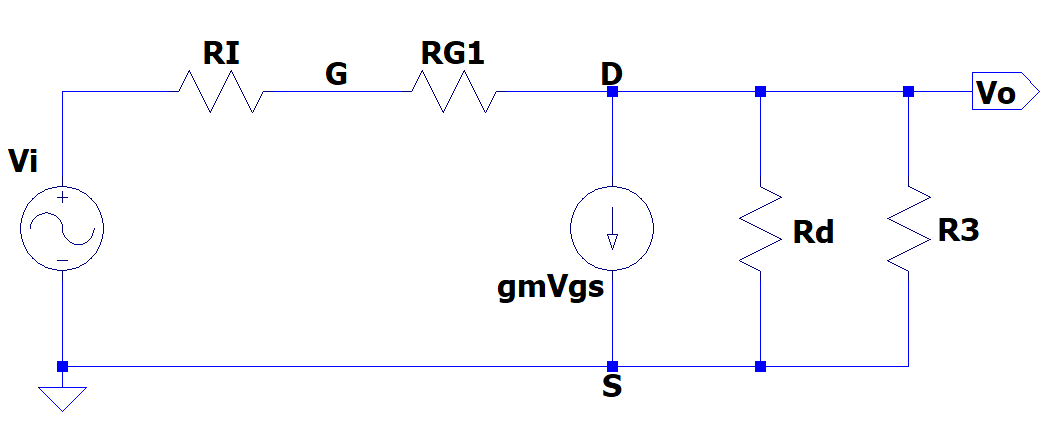
\includegraphics[width=0.5\linewidth]{es2-1-pc.png}
 	\centering
 	\caption{Circuito equivalente per piccolo segnale.}
  	\label{fig:pic1}
\end{figure}

Definiamo come prima cosa la resistenza equivalente \textit{R$_L$} (uguale al parallelo delle resistenze R$_D$ ed R$_3$) e le correnti \textit{i$_I$} (corrente che scorre nel ramo del generatore di ingresso) e \textit{i$_{//}$} (corrente che scorre nel ramo della resistenza R$_L$). Per la legge di Kirchhoff delle correnti applicata al nodo D, risulta essere vera l'eguaglianza
\begin{align*}
i_{//} = i_I - g_m v_{gs}
\end{align*}
La tensione in uscita V$_o$ puo' quindi essere definita come
\begin{equation}
\label{eq1}
v_o = i_{//}\cdot R_L = (i_I - g_m v_{gs})\cdot R_L = \left(\frac{v_I - v_o}{R_I+R_{G1}} - g_m v_{gs}\right) \cdot R_L
\end{equation}
dove la corrente i$_I$ e' stata calcolata come rapporto tra differenza potenziale in ingresso - potenziale in uscita e la serie delle resistenze R$_I$ e R$_{G1}$. La differenza di potenziale v$_{gs}$ puo' a sua volta essere scritta in funzione del segnale in ingresso v$_I$
\begin{equation}
\label{eq2}
v_{gs} = v_I - i_I \cdot R_I
\end{equation}
Unendo tra loro le relazioni (\ref{eq2}) e (\ref{eq1}) troviamo una nuova relazione in funzione delle sole incognite v$_o$ e v$_I$
\begin{equation*} \label{ol}
\begin{split}
v_o & = (i_I - g_m(v_I-i_I R_I))\cdot R_L \\
& = (i_I(1 + g_mR_I)-g_mv_I)\cdot R_L \\
& = \left( \frac{v_I-v_o}{R_I+R_{G1}} \cdot (1+g_mR_I) - g_m v_I \right) \cdot R_L 
\end{split}
\end{equation*}

\noindent Raggruppando i due termini troviamo la relazione
\begin{equation}
\label{eq3}
v_o \cdot \left( 1 + \frac{(1+g_mR_I)\cdot R_L}{R_I+R_{G1}} \right) = v_I \cdot (1-g_mR_G) \frac{R_L}{R_I+R_{G1}}
\end{equation}
A partire dalla relazione (\ref{eq3}), possiamo infine scrivere il guadagno come
\begin{equation*}
A_V = \frac{v_o}{v_I} = \frac{(1-g_mR_{G1})\cdot \frac{R_L}{R_I+R_{G1}}}{1+\frac{(1+g_mR_I)\cdot R_L}{R_I+R_{G1}}} = -13.44 \ \frac{V}{V}
\end{equation*}

Il calcolo della resistenza R$_{in}$ in ingresso all'amplificatore e' stato svolto togliendo le componenti relative al generatore di segnale in ingresso (v$_I$ e R$_I$) e sostituendole con un generatore di tensione ideale di prova V$_x$ (attraversato da una corrente i$_x$). Sia R$_L$ la resistenza equivalente al parallelo di R$_3$ e R$_D$.
Per la legge di Kirchhoff delle correnti applicata al drain del transistor abbiamo che
\begin{equation*}
i_x = g_mv_{gs} + \frac{v_o}{R_L} = g_mV_x+ \frac{V_x}{R_L} - i_x\frac{R_{G1}}{R_L}
\end{equation*}
Possiamo scrivere quindi la corrente i$_x$ in funzione della tensione V$_x$
\begin{equation*}
i_x = V_x \cdot \left( \frac{g_m+\frac{1}{R_L}}{1+\frac{R_{G1}}{R_L}} \right)
\end{equation*}
La resistenza in ingresso all'amplificatore risulta quindi essere
\begin{equation*}
R_{in} = \frac{V_x}{i_x} = \frac{1+\frac{R_{G1}}{R_L}}{g_m + \frac{1}{R_L}} = 72\,961\Omega
\end{equation*}

Per quanto riguarda invece il calcolo della resistenza in uscita, e' stato cortocircuitato il generatore del segnale in ingresso ed e' stata tolta la resistenza R$_3$. Sono in questo caso definite le correnti \textit{i'} (corrente che scorre nel ramo della resistenza R$_{G1}$) e \textit{i''} (corrente che scorre nel ramo di R$_D$) nel seguente modo
\begin{gather*}
i\,' = \frac{V_x}{R_{G1}+R_I}  \qquad \qquad i\,''=\frac{V_x}{R_D}
\end{gather*}
Per la legge di Kirchhoff delle correnti applicata al drain abbiamo che 
\begin{equation*}
i_x = \frac{V_x}{R_{G1}+R_I} +  \frac{V_x}{R_D} + \frac{g_mV_xR_I}{R_I+R_{G1}} = V_x \cdot \left( \frac{R_D+R_{G1}+R_I+g_mR_IR_D}{(R_{G1}+R_I)R_D} \right)
\end{equation*}
per cui la resistenza in uscita diventa
\begin{equation*}
R_{out} = \frac{V_x}{i_x} = \frac{R_D(R_{G1}+R_I)}{R_DR_{G1}+R_I+g_mR_IR_D} = 87.69\Omega
\end{equation*}

\newpage

\subsubsection{Simulare con SPICE il punto operativo del circuito e verificare i valori trovati analiticamente}
Il listato SPICE utilizzato per simulare il punto operativo del circuito e' riportato di seguito
\begin{verbatim}
* Esercizio 2.1
* input
Vi in 0 AC 1 SINE(0 100m 1K)
Ri N3 in 10k
C1 vG N3 1000u
* RG
RG1 vD vG 1187180
* altri componenti
Rd vD N1 100
R3 0 out 1k
C2 out vD 1000u
Vdd N1 0 5
M1 vD vG 0 0 NMOS
.model NMOS NMOS LEVEL=1 VTO=1 KP=8m W=100u L=2u
.op
.end
\end{verbatim}
Il risultato di questa analisi fornisce in output i seguenti dati (sono riportati solo i valori significativi che dovevano essere confrontati con i risultati analitici). Tutti i risultati della simulazione coincidono con quelli calcolati analiticamente.
\begin{verbatim}
V(vd):	 1.42291	 voltage
V(vg):	 1.42291	 voltage
Id(M1):	 0.035771	 device_current
\end{verbatim}
\newpage

\subsubsection{Con f(v$_I$) = 1kHz, simulare con SPICE 10 periodi di v$_I$, v$_o$; simulare il guadagno e confrontare il valore ottenuto con i risultati analitici}
Il comportamento dei segnali di ingresso e uscita nei loro primi 10 periodi e' riportato in figura (Figure \ref{fig:inout1}). L'andamento del guadagno nei primi 10 periodi di e' invece riportato successivamente (Figure \ref{fig:gain10}). Infine, e' riportato un grafico in cui si evidenzia il guadagno in funzione della frequenza del segnale in ingresso (Figure \ref{fig:gainfreq}).

\begin{figure}[h!]
  	\centering
 	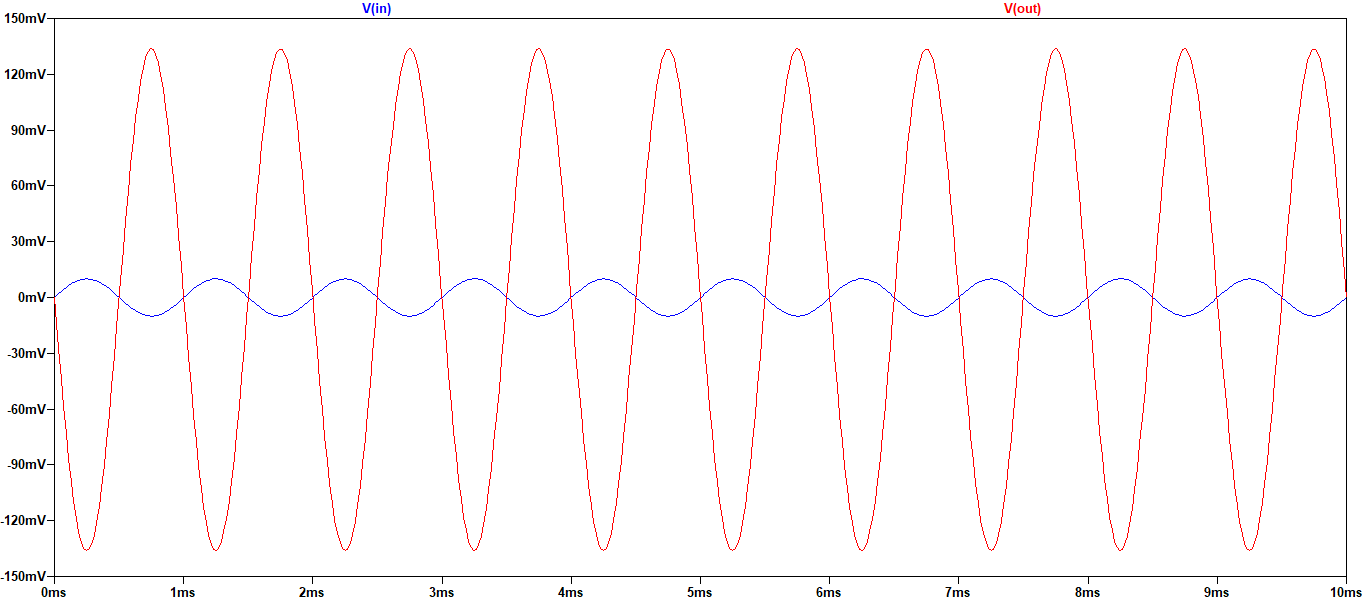
\includegraphics[width=0.7\linewidth]{es2-1-5-1.png}
  	\caption{Andamento segnali ingresso e uscita nei primi 10 periodi.}
  	\label{fig:inout1}
\end{figure}
\begin{figure}[h!]
  	\centering
 	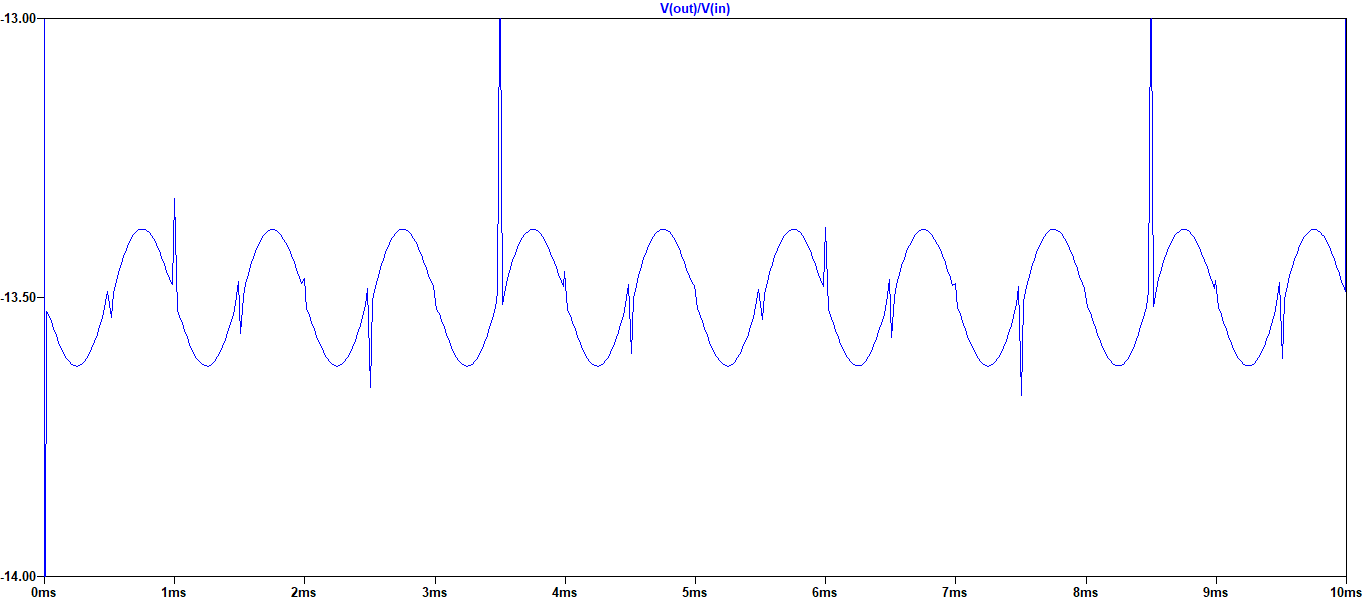
\includegraphics[width=0.7\linewidth]{es2-1-5bis.png}
  	\caption{Andamento del guadagno dell'amplificatore nei primi 10 periodi.}
  	\label{fig:gain10}
\end{figure}
\begin{figure}[h!]
  	\centering
 	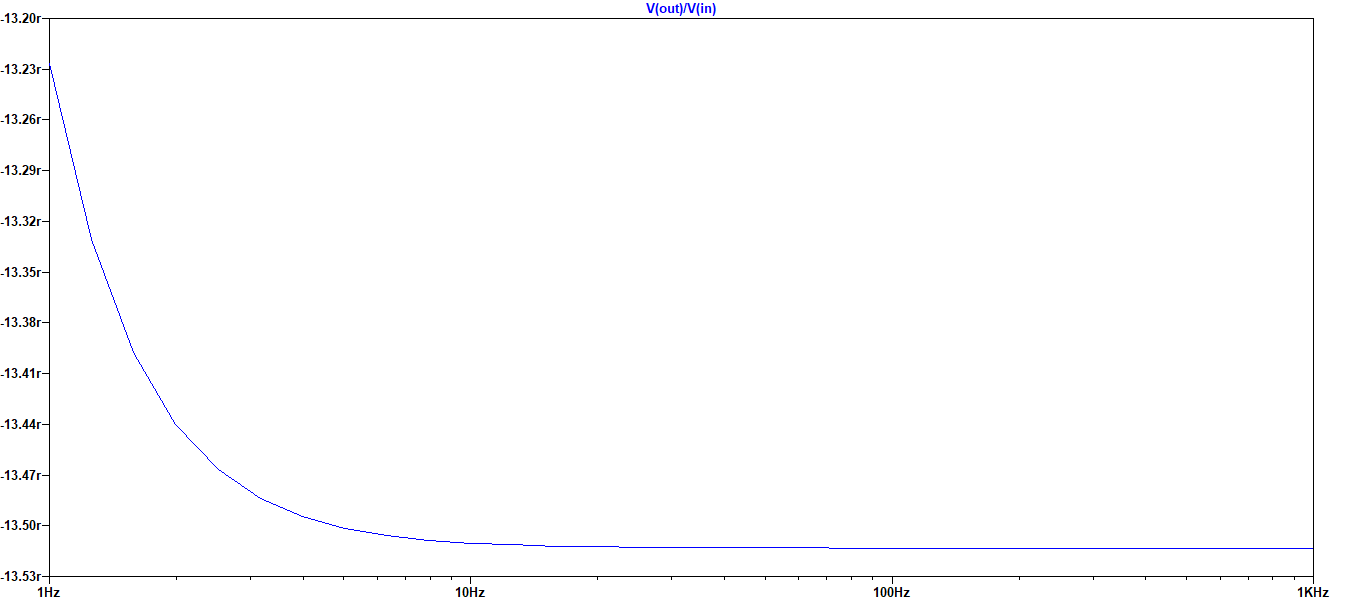
\includegraphics[width=0.7\linewidth]{es2-1-5.png}
  	\caption{Guadagno dell'amplificatore in funzione della frequenza del segnale di ingresso.}
  	\label{fig:gainfreq}
\end{figure}
I valori ritrovati in queste simulazioni coincidono con quelli trovati analiticamente, al netto di leggeri scostamenti (inferiori all'1\%) sul valore del guadagno, dovuti molto probabilmente all'approssimazione nei calcoli. Il transitorio a basse frequenze invece e' un effetto dovuto al filtraggio attuato dai condensatori.
\newpage

\subsubsection{Ripetere il punto 1.5 con ampiezza del segnale v$_I$ pari a 100 mV: spiegare cosa avviene}
Nel caso in cui l'ampiezza del segnale in ingresso sia fissata a 100mV, le caratteristiche che ne derivano sono riportate di seguito (nello stesso ordine dell'esercizio precedente).
\begin{figure}[h!]
  	\centering
 	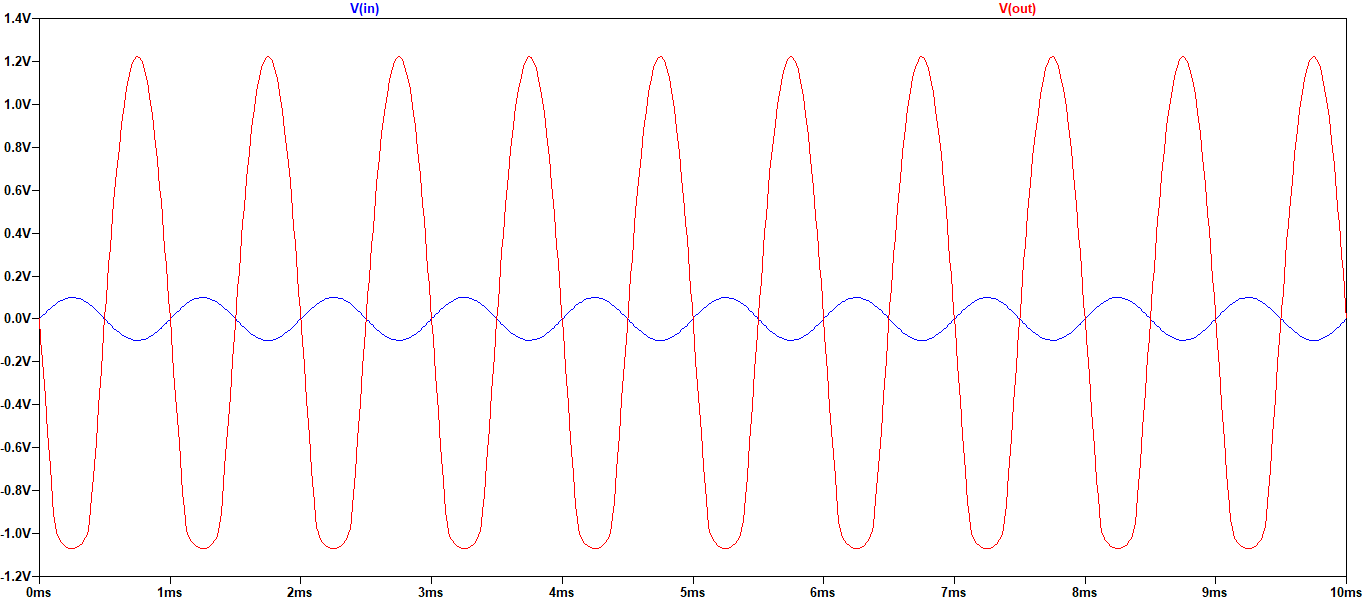
\includegraphics[width=0.67\linewidth]{es2-1-6inout.png}
  	\caption{Andamento segnali ingresso e uscita nei primi 10 periodi.}
  	\label{fig:inout2}
\end{figure}
\begin{figure}[h!]
  	\centering
 	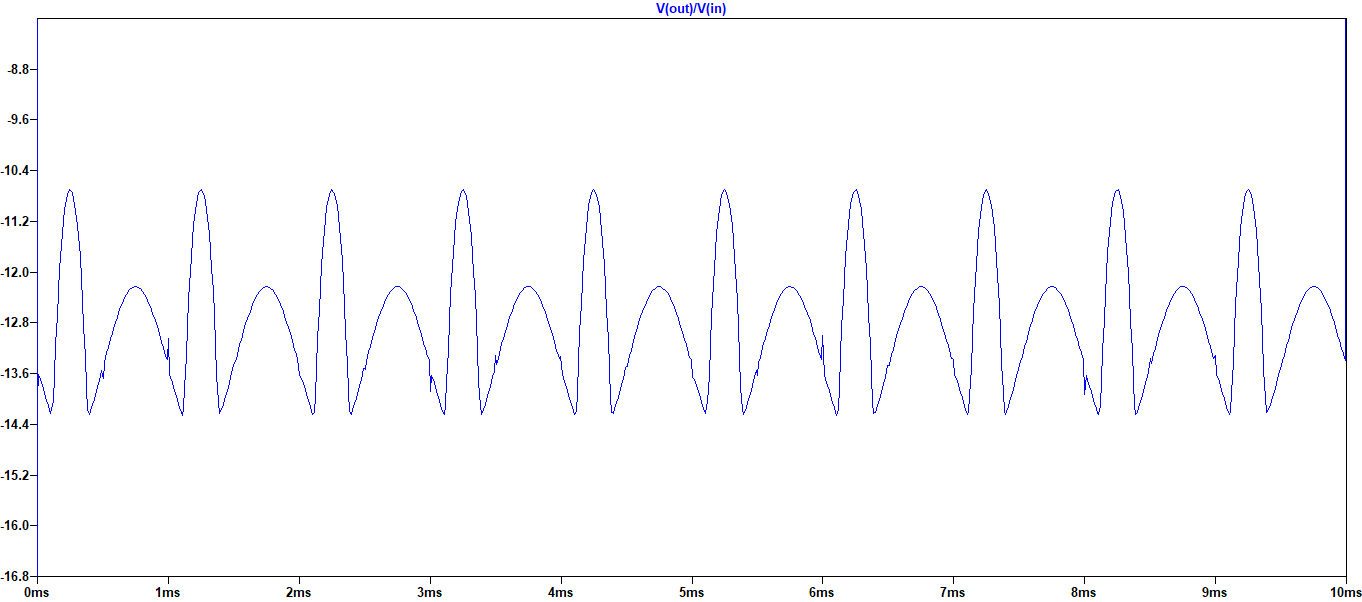
\includegraphics[width=0.67\linewidth]{es2-1-6.png}
  	\caption{Andamento del guadagno dell'amplificatore nei primi 10 periodi.}
  	\label{fig:gain100}
\end{figure}
\begin{figure}[h!]
  	\centering
 	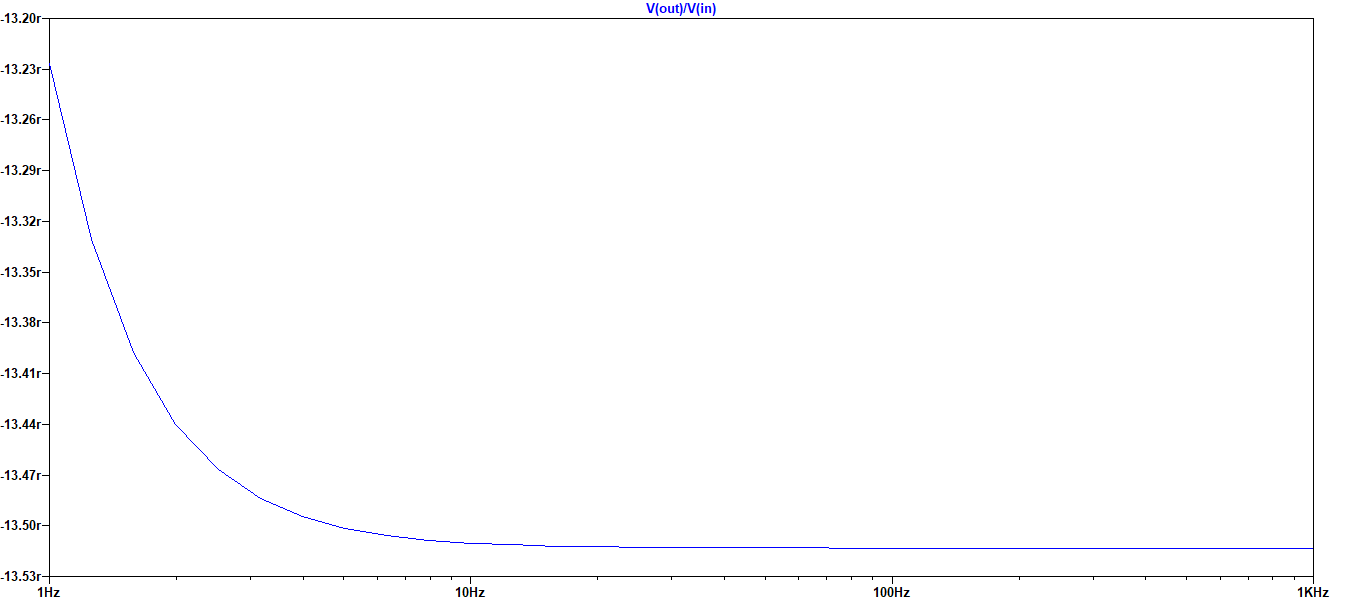
\includegraphics[width=0.67\linewidth]{es2-1-6bis.png}
  	\caption{Guadagno dell'amplificatore in funzione della frequenza del segnale di ingresso.}
  	\label{fig:gainfreq2}
\end{figure}

Le differenze che possiamo notare tra la precedente situazione e questa riguardano i primi due grafici. Il comportamento anomalo e' molto marcato nel grafico del guadagno in funzione del tempo, mentre lo e' un po' meno (seppur sempre apprezzabile visivamente) nel grafico della tensione di uscita (in corrispondenza dei picchi positivi del segnale in ingresso). Il fenomeno che si osserva in questo caso e' quello dell'uscita del diodo dalla condizione di saturazione: l'ampiezza del segnale in ingresso (che influenza direttamente la tensione di gate che polarizza il MOS) diventa infatti in certi tratti cosi' grande da pregiudicare la validita' della condizione di saturazione \textit{V$_{DS} + v_{ds} > V_{GS} + v_{gs} - V_{tn}$}. 

\subsubsection{Calcolare e verificare tramite simulazioni il massimo valore dell'ampiezza del segnale v$_I$ che garantisce una risposta lineare dell'amplificatore}
Affinche' la risposta dell'amplificatore sia lineare, devono essere rispettate due condizioni:
\begin{itemize}
 	\item \textit{$v_{gs} << 2(V_{GSQ}-V_{tn})$}, ovvero la condizione che deriva dalla linearizzazione della dipendenza tra tensione di gate e corrente di drain (che sarebbe di tipo quadratico)
 	\item \textit{$V_{DSQ} + v_{ds,min} > V_{GSQ}+v_{gs,max}-V_{tn}$}, che deriva invece dall'ipotesi di funzionamento in saturazione del transistor 
\end{itemize}
Tra le due condizioni, la piu' stringente risulta essere la seconda. Possiamo riscriverla, dopo aver trovato che $v_{gs}=0.89v_I$, come
\begin{gather*}
V_{DSQ} + v_{ds,min} = V_{DSQ} - |A_v|v_{I,max} > V_{GSQ}+v_{gs,max}-V_{tn} \\
-|A_v|v_{I,max} > 0.89v_{I,max} - V_{tn} \\
v_{I,max} < \frac{V_{tn}}{|A_v|+0.89} = 69.78mV
\end{gather*}
Tramite simulazioni invece il massimo valore di ampiezza che garantisce il funzionamento lineare risulta essere $\approx 66mV$, ricavato dal grafico riportato (Figure \ref{fig:effettodi}). La discrepanza tra valore trovato analiticamente e valore osservato sperimentalmente puo' essere spiegata dalla presenza di uno stato di transizione terzo alla saturazione e alla linearita', in cui il comportamento della corrente di drain e' una via di mezzo tra i due comportamenti che congiunge.
\begin{figure}[h!]
  	\centering
 	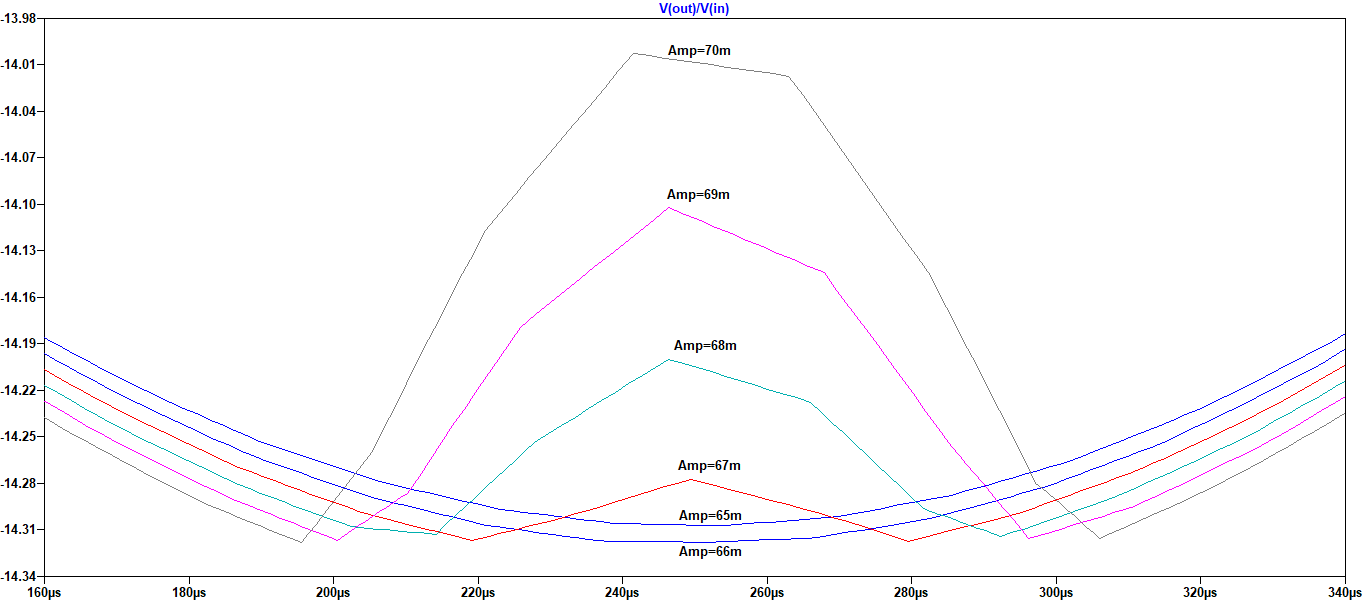
\includegraphics[width=0.67\linewidth]{es2-1-7gain.png}
  	\caption{Guadagno dell'amplificatore in funzione della frequenza del segnale di ingresso.}
  	\label{fig:effettodi}
\end{figure}
\newpage


\subsection{Porre R$_{G1}$=R$_{G2}$ pari al proprio numero di matricola}

\subsubsection{Calcolare analiticamente il punto di polarizzazione DC del transistor}
Per prima cosa, disegniamo il circuito equivalente nell'analisi a largo segnale (Figure \ref{fig:pol2}), in cui tutti i condensatori equivalgono a circuiti aperti e tutti i segnali non DC sono annullati.

\begin{figure}[h!]
 	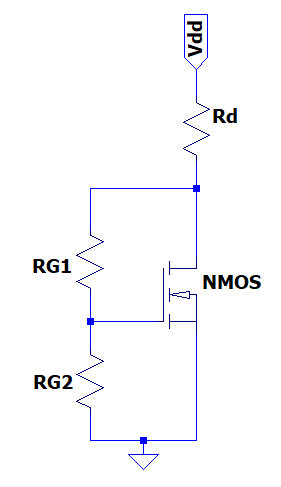
\includegraphics[width=0.16\linewidth]{pol2.png}
 	\centering
 	\caption{Circuito equivalente per largo segnale.}
  	\label{fig:pol2}
\end{figure}

D'ora in avanti consideriamo nei calcoli la resistenza $R_G=R_{G1}=R_{G2}$. La tensione V$_{GSQ}$ in queste condizioni diventa (per il partitore di tensione sulle due resistenze R$_{G1}$ e R$_{G2}$)
\begin{equation*}
V_{GSQ} = V_{DSQ} \cdot \frac{R_{G}}{R_{G}+R_G} = 0.5 V_{DSQ}
\end{equation*}
Ipotizziamo che il transistor si trovi in saturazione. Mettendo a sistema la relazione della corrente di drain in saturazione e la legge di Kirchoof delle tensioni applicata alla maglia V$_{DD}$-R$_D$-MOS si ha
\begin{align*}
	\begin{cases}
		I_{DQ} = \frac{k_n}{2} \cdot (\frac{V_{DSQ}}{2}-V_{tn})^2 \\[4pt]
		V_{DSQ} = \frac{V_{DD}-I_DR_D}{1+\frac{R_D}{2R_G}}
	\end{cases}
\end{align*}
Lavoriamo nell'ipotesi in cui gli effetti dovuti alla corrente che scorre nella serie delle due resistenze R$_G$ sia trascurabile (da verificare). Il risultato del sistema e' un'equazione di secondo grado nell'incognita I$_{DQ}$.
\begin{align*}
100^2 I_{DQ}^2 - 620 I_{DQ} + 9 = 0 
\end{align*}
le cui soluzioni sono
\begin{align*}
I_{DQ} = 23.19mA \ \Rightarrow \  V_{GSQ} - V_{tn} = \mathbf{0.34V}  \textit{  ok}\\
I_{DQ} = 38.81mA \  \Rightarrow \ V_{GSQ} - V_{tn} = -0.44V < 0 \textit{  no}
\end{align*}
Nota $I_{DQ}$, possiamo calcolare le tensioni V$_{GSQ}$ e V$_{DSQ}$
\begin{gather*}
V_{DSQ} \approx V_{DD} - I_DR_D = 2.68V \\
V_{GSQ} \approx 0.5 \cdot V_{GSQ} = 1.34V
\end{gather*}
La corrente che scorre nel ramo della serie R$_G$ risulta quindi essere $1.129\mu A$ e l'ipotesi di trascurabilita' e' quindi verificata.
\newpage

\subsubsection{Calcolare i parametri del il modello per piccolo segnale}
Il calcolo dei parametri del modello per piccolo segnale e' riportato di seguito
\begin{align*}
g_m = k_n \cdot V_{ov} = 136mS \qquad \qquad \qquad r_o = \infty
\end{align*}

\subsubsection{Disegnare il modello per piccolo segnale dell'amplificatore e calcolare il guadagno in tensione, R$_{in}$ e R$_o$.}
Il modello per piccolo segnale dell'amplificatore a source comune in esame e' rappresentato di seguito (Figure \ref{fig:pic2}). 
\begin{figure}[h!]
 	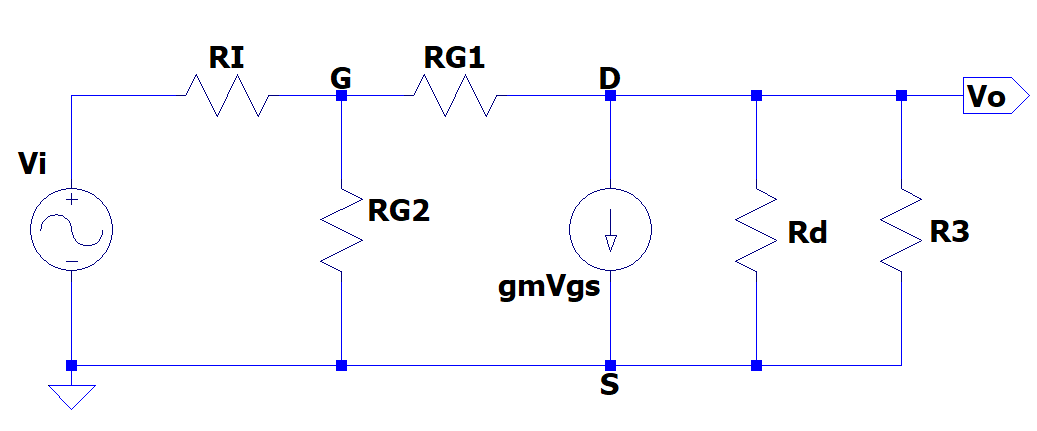
\includegraphics[width=0.5\linewidth]{es2-2-pc.png}
 	\centering
 	\caption{Circuito equivalente per piccolo segnale.}
  	\label{fig:pic2}
\end{figure}

Definiamo come prima cosa la resistenza equivalente \textit{R$_L$} (uguale al parallelo delle resistenze R$_D$ ed R$_3$) e le correnti \textit{i$_I$} (corrente che scorre nel ramo del generatore di ingresso), \textit{i$_{R2}$} (corrente che scorre nel ramo della resistenza R$_{G2}$), \textit{i$_{R1}$} (corrente che scorre nel ramo della resistenza R$_{G1}$  e \textit{i$_{//}$} (corrente che scorre nel ramo della resistenza R$_L$), che equivalgono a
\begin{equation*}
i_{R2}=\frac{v_{gs}}{R_{G}} \qquad \qquad i_{R1}=\frac{v_{gs}-v_o}{R_{G}} \qquad \qquad i_I=\frac{v_I-v_{gs}}{R_I} \qquad \qquad i_{//}=\frac{v_o}{R_L}
\end{equation*}
Applichiamo la legge di Kirchhoof delle correnti al nodo gate, trovando $i_I = i_{R1} + i_{R2}$. Possiamo quindi scrivere che 
\begin{align*}
\frac{v_I-v_{gs}}{R_I}=\frac{v_{gs}R_G-v_oR_G+v_{gs}R_G}{R_G^2}
\end{align*}
A seguito di una serie di passaggi algebrici di semplificazione, troviamo la relazione
\begin{equation}
\label{eq2-1}
v_o=v_{gs}(2+\frac{R_G}{R_I})-v_I\frac{R_G}{R_I}
\end{equation}
Applicando invece Kirchhoff delle correnti al nodo drain, abbiamo che $i_{R1} = g_mv_{gs} + i_{//}$. In questo caso, dalla legge di Ohm, troviamo che
\begin{equation*}
\frac{v_{gs}-v_o}{R_G} = \frac{g_mv_{gs}R_L+v_o}{R_L}
\end{equation*}
Anche in questo caso, a seguito di una serie di passaggi di semplificazione, possiamo riscrivere quest'ultima relazione come
\begin{equation}
\label{eq2-2}
v_{gs} = v_o \left( \frac{R_G+R_L}{R_L-g_mR_LR_G} \right)
\end{equation}
Unendo le relazioni (\ref{eq2-1}) e (\ref{eq2-2}) precedentemente ricavate troviamo che
\begin{equation*}
v_o=v_o\left(\frac{R_G+R_L}{R_L-g_mR_LR_G}\right)\left(2+\frac{R_G}{R_I}\right)-v_I\frac{R_G}{R_I}
\end{equation*}
Per cui il guadagno in tensione dell'amplificatore puo' essere calcolato come
\begin{equation}
\label{eq2-3}
A_v=\frac{v_o}{v_I} = \frac{-\frac{R_G}{R_I}}{1-\left(\frac{R_G+R_L}{R_L-g_mR_LR_G}\right)\left(2+\frac{R_G}{R_I}\right)} = -11.038\ \frac{V}{V}
\end{equation}

Il calcolo della resistenza R$_{in}$ in ingresso all'amplificatore e' stato svolto togliendo le componenti relative al generatore di segnale in ingresso (v$_I$ e R$_I$) e sostituendole con un generatore di tensione ideale di prova V$_x$ (attraversato da una corrente i$_x$). Sia R$_L$ la resistenza equivalente al parallelo di R$_3$ e R$_D$. Siano i$_G1$ e i$_G2$ le correnti che attraversano le rispettive R$_G$.
Per la legge di Kirchhoff delle correnti applicata al drain del transistor abbiamo che
\begin{equation*}
i_{G1} = g_mv_{gs} + \frac{v_o}{R_L} = g_mV_x+ \frac{V_x-i_{G1}R_G}{R_L} \quad \Rightarrow \quad i_{G1} = V_x \frac{\left(g_m+\frac{1}{R_L}\right)}{\left(1+\frac{R_G}{R_L}\right)}
\end{equation*}
Applicando ora la legge di Kirchhoff delle correnti al gate troviamo che
\begin{equation*}
i_x=\frac{V_x}{R_G}+V_x\frac{g_m+\frac{1}{R_L}}{1+\frac{R_G}{R_L}} = V_x \left( \frac{1}{R_G} + \frac{g_m+\frac{1}{R_L}}{1+\frac{R_G}{R_L}} \right)
\end{equation*}
La resistenza in ingresso all'amplificatore risulta quindi essere
\begin{equation}
\label{eq2-4}
R_{in} = \frac{V_x}{i_x} = \frac{1}{\frac{1}{R_G} + \frac{g_m+\frac{1}{R_L}}{1+\frac{R_G}{R_L}}} = 82\,586\Omega
\end{equation}

Per quanto riguarda invece il calcolo della resistenza in uscita, e' stato cortocircuitato il generatore del segnale in ingresso ed e' stata tolta la resistenza R$_3$. E' definita la resistenza $R_p=R_I//R_{G2}$. Sono inoltre definite le correnti \textit{i$_{//}$} (corrente che scorre nel ramo della resistenza R$_{G1}$) e \textit{i$_D$} (corrente che scorre nel ramo di R$_D$) nel seguente modo
\begin{gather*}
i_{G1} = \frac{V_x}{R_{G1}+R_p}  \qquad \qquad i_D=\frac{V_x}{R_D}
\end{gather*}
Per la legge di Kirchhoff delle correnti applicata al drain abbiamo che 
\begin{equation*}
i_x = \frac{V_x}{R_{G1}+R_p}+V_x\frac{g_mR_p}{R_{G1}+R_p}+\frac{V_x}{R_D}
\end{equation*}
per cui la resistenza in uscita diventa
\begin{equation}
\label{eq2-5}
R_{out} = \frac{V_x}{i_x} = \frac{(R_{G1}+R_p)R_D}{R_D+g_mR_DR_p+R_{G1}+R_p} = 89.87\Omega
\end{equation}

\newpage

\subsubsection{Simulare con SPICE il punto operativo del circuito e verificare i valori trovati analiticamente}
Il listato SPICE utilizzato per simulare il punto operativo del circuito e' riportato di seguito
\begin{verbatim}
* Esercizio 2.2
* input
Vi in 0 SINE(0 10m 1K)
Ri N3 in 10k
C1 vG N3 1000u
* RG
RG1 vD vG 1187180
RG2 vG 0 1187180
* altri componenti
Rd vD N1 100
R3 0 out 1k
C2 out vD 1000u
Vdd N1 0 5
M1 vD vG 0 0 NMOS
.model NMOS NMOS LEVEL=1 VTO=1 KP=8m W=100u L=2u
.op
.end
\end{verbatim}
Il risultato di questa analisi fornisce in output i seguenti dati (sono riportati solo i valori significativi che dovevano essere confrontati con i risultati analitici). Tutti i risultati della simulazione coincidono con quelli calcolati analiticamente.
\begin{verbatim}
V(vg):	 1.34051	 voltage
V(vd):	 2.68101	 voltage
Id(M1):	 0.0231888	 device_current
I(Rg2):	 1.12915e-006	 device_current
\end{verbatim}
\newpage

\subsubsection{Con f(v$_I$) = 1kHz, simulare con SPICE 10 periodi di v$_I$, v$_o$; simulare il guadagno e confrontare il valore ottenuto con i risultati analitici}
Il comportamento dei segnali di ingresso e uscita nei loro primi 10 periodi e' riportato in figura (Figure \ref{fig:inout2}). L'andamento del guadagno nei primi 10 periodi di e' invece riportato successivamente (Figure \ref{fig:gain10-2}). Infine, e' riportato un grafico in cui si evidenzia il guadagno in funzione della frequenza del segnale in ingresso (Figure \ref{fig:gainfreq-2}).

\begin{figure}[h!]
  	\centering
 	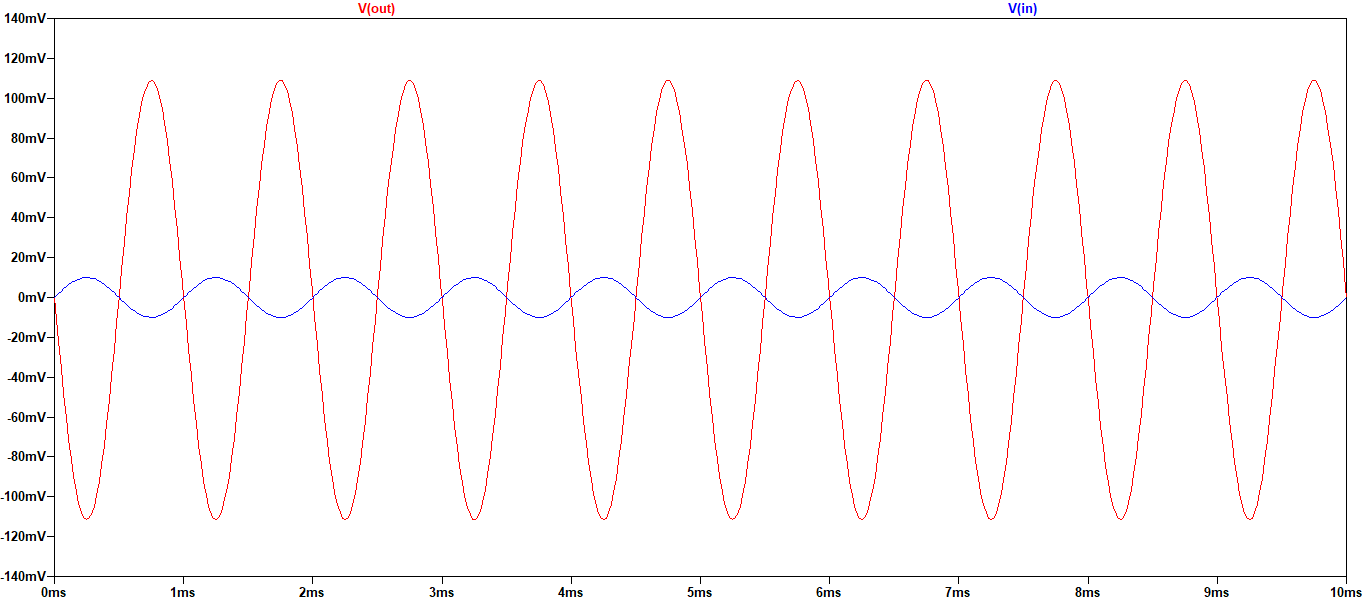
\includegraphics[width=0.7\linewidth]{es2-2-3sign.png}
  	\caption{Andamento segnali ingresso e uscita nei primi 10 periodi.}
  	\label{fig:inout2}
\end{figure}
\begin{figure}[h!]
  	\centering
 	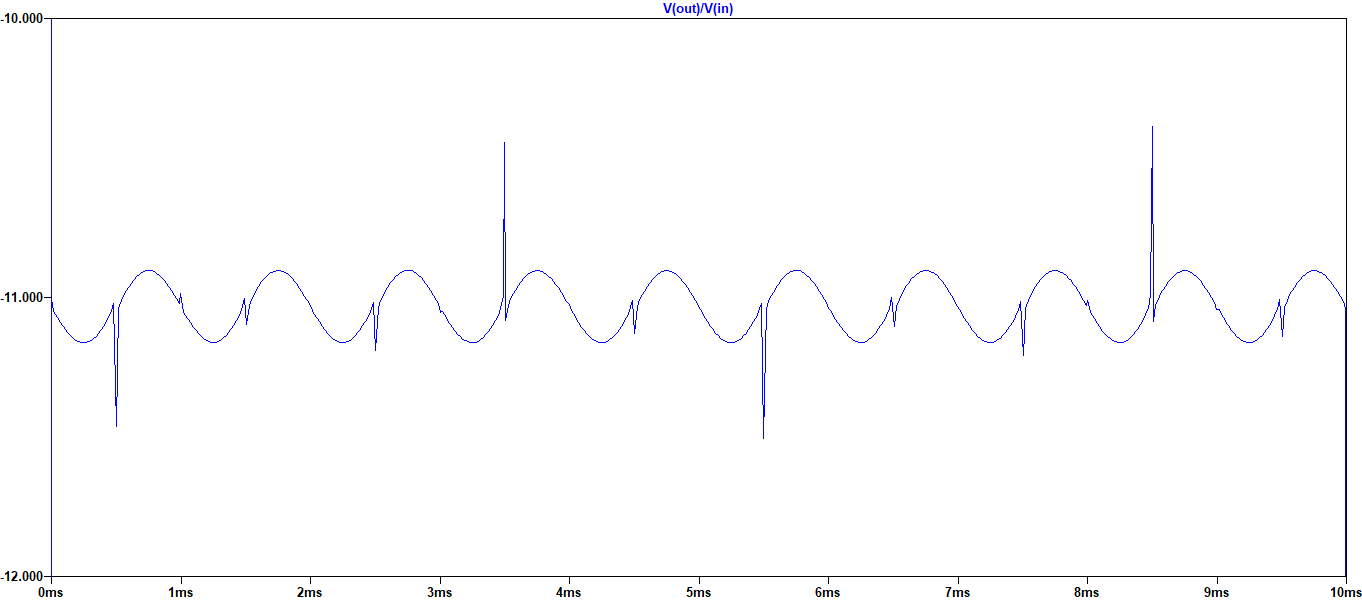
\includegraphics[width=0.7\linewidth]{es2-2-3gain.png}
  	\caption{Andamento del guadagno dell'amplificatore nei primi 10 periodi.}
  	\label{fig:gain10-2}
\end{figure}
\begin{figure}[h!]
  	\centering
 	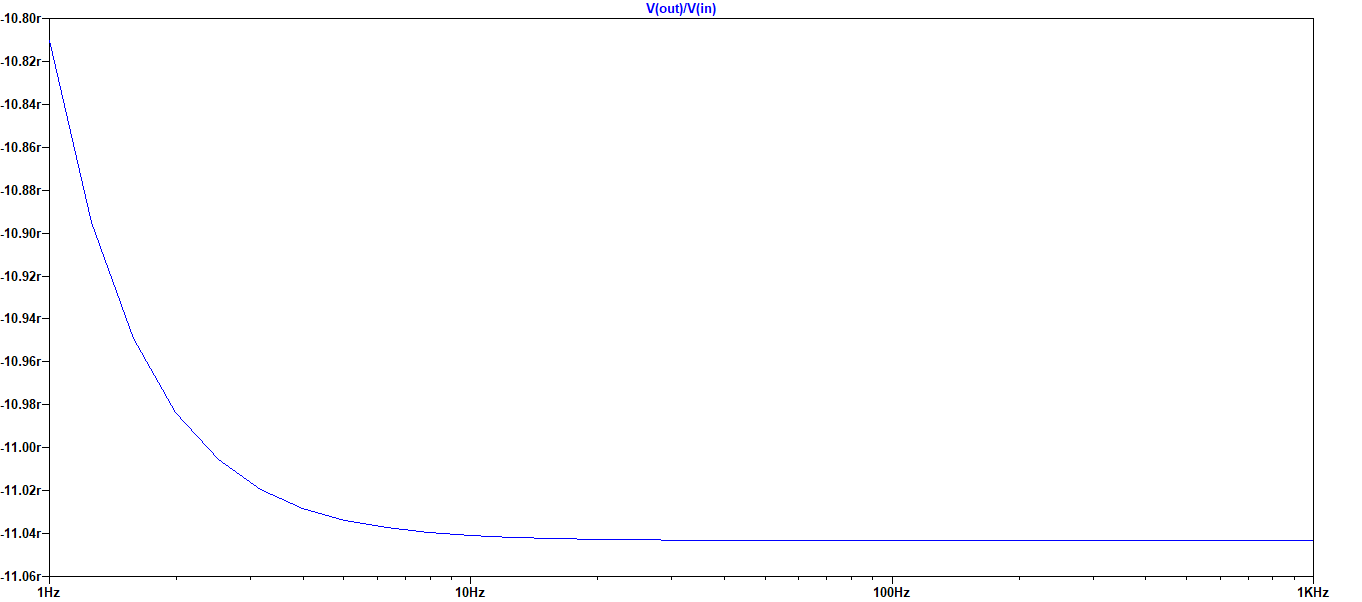
\includegraphics[width=0.7\linewidth]{es2-2-3freq.png}
  	\caption{Guadagno dell'amplificatore in funzione della frequenza del segnale di ingresso.}
  	\label{fig:gainfreq-2}
\end{figure}
I valori ritrovati in queste simulazioni coincidono con quelli trovati analiticamente. Il transitorio a basse frequenze invece e' un effetto dovuto al filtraggio attuato dai condensatori.

\newpage

\subsubsection{Calcolare e verificare tramite simulazioni il massimo valore dell'ampiezza del segnale v$_I$ che garantisce una risposta lineare dell'amplificatore}
Affinche' la risposta dell'amplificatore sia lineare, devono essere rispettate due condizioni:
\begin{itemize}
 	\item \textit{$v_{gs} << 2(V_{GSQ}-V_{tn})$}, ovvero la condizione che deriva dalla linearizzazione della dipendenza tra tensione di gate e corrente di drain (che sarebbe di tipo quadratico)
 	\item \textit{$V_{DSQ} + v_{ds,min} > V_{GSQ}+v_{gs,max}-V_{tn}$}, che deriva invece dall'ipotesi di funzionamento in saturazione del transistor 
\end{itemize}
Tra le due condizioni, la piu' stringente risulta essere la seconda. Possiamo riscriverla come
\begin{gather*}
V_{DSQ} + v_{ds,min} = V_{DSQ} - |A_v|v_{I,max} > V_{GSQ}+v_{gs,max}-V_{tn} 
\end{gather*}
Troviamo che $v_{gs}=v_I\frac{2R_G-11R_I}{2R_I+2R_G}$, per cui
\begin{gather*}
-|A_v|v_{I,max} > \frac{2R_G-11R_I}{2R_I+2R_G}v_{I,max} - V_{tn} \\
v_{I,max} < \frac{V_{GSQ}+V_{tn}}{|A_v|+0.94} = 194.87mV
\end{gather*}
Tramite simulazioni invece il massimo valore di ampiezza che garantisce il funzionamento lineare risulta essere $\approx 168mV$, ricavato dal grafico riportato (Figure \ref{fig:effettodi2}). La discrepanza tra valore trovato analiticamente e valore osservato sperimentalmente puo' essere spiegata dalla presenza di uno stato di transizione terzo alla saturazione e alla linearita', in cui il comportamento della corrente di drain e' una via di mezzo tra i due comportamenti che congiunge.
\begin{figure}[h!]
  	\centering
 	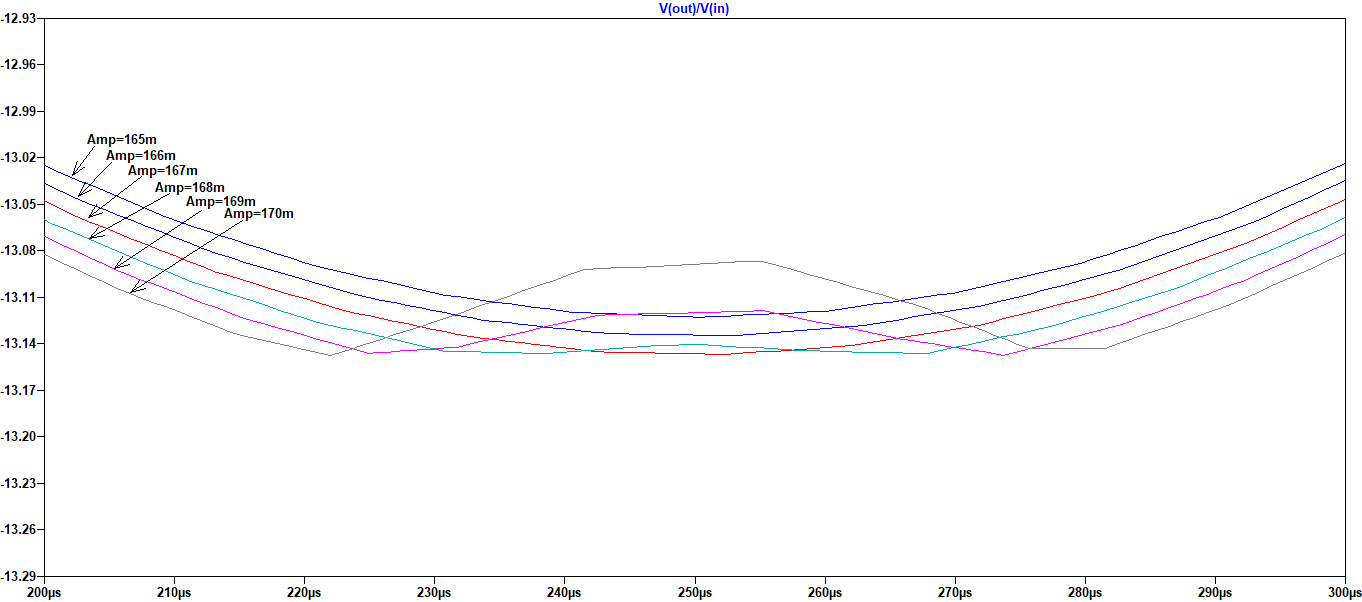
\includegraphics[width=0.67\linewidth]{es2-2-6gain.png}
  	\caption{Guadagno dell'amplificatore in funzione della frequenza del segnale di ingresso.}
  	\label{fig:effettodi2}
\end{figure}
\newpage

\subsection{Porre W=L=10$\mu$m, k'$_n$=8mA/V$^2$, V$_{tn}$=1V}

\subsubsection{Riprogettare il circuito (R$_{G1}$, R$_{G2}$ e R$_D$) in modo che la corrente di drain sia I$_D$=1mA, che V$_{DSQ}$ = V$_{OV}$ + 2V, e che la corrente attraverso R$_{G1}$ e R$_{G2}$ sia 100nA}
Il circuito equivalente per largo segnale dell'amplificatore non cambia rispetto a quello del punto precedente (Figure \ref{fig:pol2}). Cominciamo con la riprogettazione del circuito sulla base dei dati forniti. Sapendo che 
\begin{equation*}
V_{DS} - V_{GS} = V_D - V_G = 1V
\end{equation*}
possiamo calcolare la resistenza R$_{G1}$ come
\begin{equation*}
R_{G1} = \frac{V_D-V_G}{I_{RG}} = 10 \,M\Omega
\end{equation*}
dove I$_{RG}$ e' la corrente che attraversa le due resistenze R$_{G1}$ e R$_{G2}$. Ipotizziamo a questo punto che il MOSFET si trovi in condizione di saturazione. Dalla relazione della corrente di drain possiamo quindi ricavare il valore della tensione di overdrive V$_{ov}$ e di conseguenza della tensione V$_{GS}$
\begin{equation*}
I_D=\frac{k_n}{2}(V_{GS}-V_{tn})^2 \qquad \Rightarrow \qquad V_{ov}=\sqrt{\frac{2I_D}{k_n}} = 0.5V
\end{equation*}
Siamo quindi in grado di trovare i valori di R$_{G2}$, V$_{GS}$ e V$_{DS}$
\begin{equation*}
V_{GS}=V_{ov}+V_{tn}=1.5V \qquad \qquad V_{DS} = V_{GS}+1V =2.5V \qquad \qquad R_{G2}=\frac{V_{GS}}{I_{RG}} = 15\, M\Omega
\end{equation*}
Infine, e' possibile trovare anche il valore della resistenza di drain
\begin{equation*}
R_D=\frac{V_{DD}-V_{DS}}{I_D} = 2500\, \Omega
\end{equation*}
Calcoliamo ora i parametri del modello per piccolo segnale
\begin{equation*}
g_m=k_n(V_{GS}-V_{tn}) = 4mS \qquad\qquad r_o=\infty
\end{equation*}
Il modello per piccolo segnale in questo caso e' perfettamente equivalente a quello del punto precedente (Figure \ref{fig:pic2}), al netto delle variazioni dei valori di tensione, corrente e resistenza. Per questo motivo possiamo riutilizzare anche le relazioni per il calcolo di guadagno, R$_{in}$ e R$_{out}$. \\ \\
Per (\ref{eq2-3}) il guadagno in tensione dell'amplificatore risulta essere $A_v=-2.843\,\frac{V}{V}$. Per (\ref{eq2-4}) invece la resistenza in ingresso all'amplificatore risulta $R_{in}=2.211\,M\Omega$, mentre per (\ref{eq2-5}) si ha che $R_{out}=2472\,\Omega$.

\newpage
\subsubsection{Simulare con SPICE il punto operativo del circuito e verificare i valori trovati analiticamente}
Il listato SPICE utilizzato per simulare il circuito e' riportato di seguito.
\begin{verbatim}
* Esercizio 2.3
* input
Vi in 0 AC SINE(0 100m 1K)
Ri N3 in 10k
C1 vG N3 1000u
* RG
RG1 vD vG 10Meg
RG2 0 vG 15Meg
* altri componenti
Rd vD N1 2.5k
R3 0 out 1k
C2 out vD 1000u
Vdd N1 0 5
M1 vD vG 0 0 NMOS
.model NMOS NMOS LEVEL=1 VTO=1 KP=8m W=10u L=10u
.op
.backanno
.end
\end{verbatim}
Il risultato di questa analisi fornisce in output i seguenti dati (sono riportati solo i valori significativi che dovevano essere confrontati con i risultati analitici). Tutti i risultati della simulazione coincidono con quelli calcolati analiticamente.
\begin{verbatim}
V(vg):	 1.49998	 voltage
V(vd):	 2.49996	 voltage
Id(M1):	 0.000999914	 device_current
I(Rg1):	 9.99986e-008	 device_current
\end{verbatim}
\newpage

\subsubsection{Con f(v$_I$) = 1 kHz, simulare con SPICE 10 periodi di v$_I$, v$_{out}$; simulare Av e confrontare il valore ottenuto con i risultati analitici}
Il comportamento dei segnali di ingresso e uscita nei loro primi 10 periodi e' riportato in figura (Figure \ref{fig:inout3}). L'andamento del guadagno nei primi 10 periodi di e' invece riportato successivamente (Figure \ref{fig:gain10-3}). Infine, e' riportato un grafico in cui si evidenzia il guadagno in funzione della frequenza del segnale in ingresso (Figure \ref{fig:gainfreq-3}).

\begin{figure}[h!]
  	\centering
 	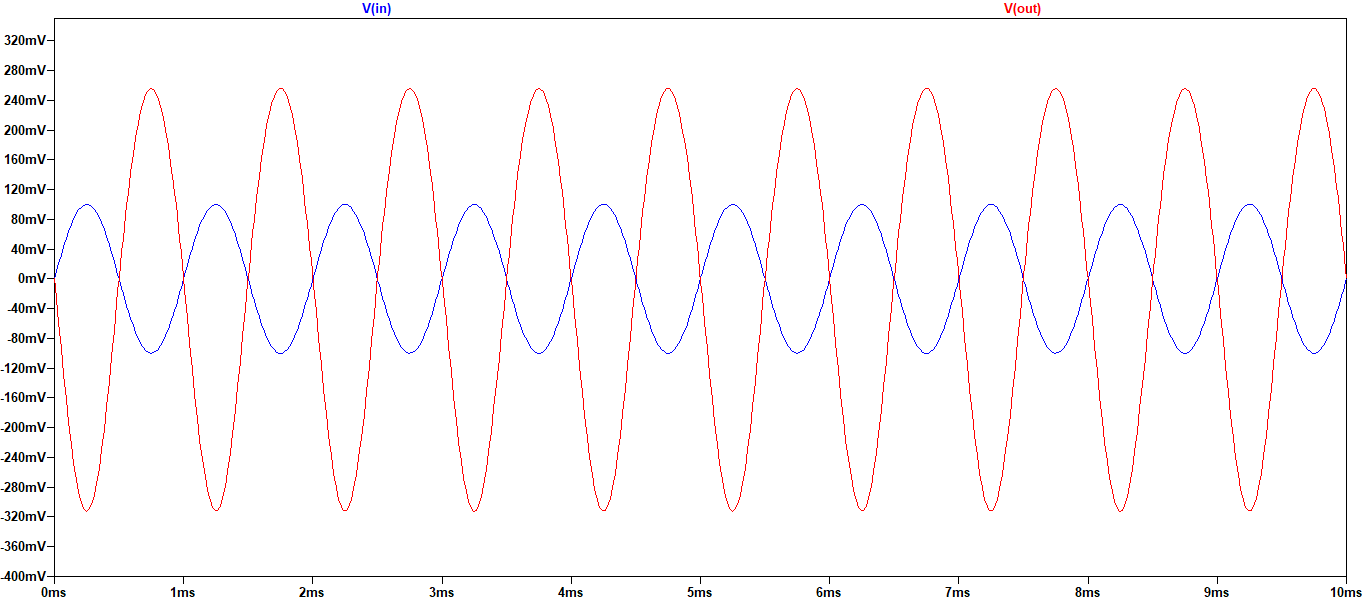
\includegraphics[width=0.7\linewidth]{es2-3-3sign.png}
  	\caption{Andamento segnali ingresso e uscita nei primi 10 periodi.}
  	\label{fig:inout3}
\end{figure}
\begin{figure}[h!]
  	\centering
 	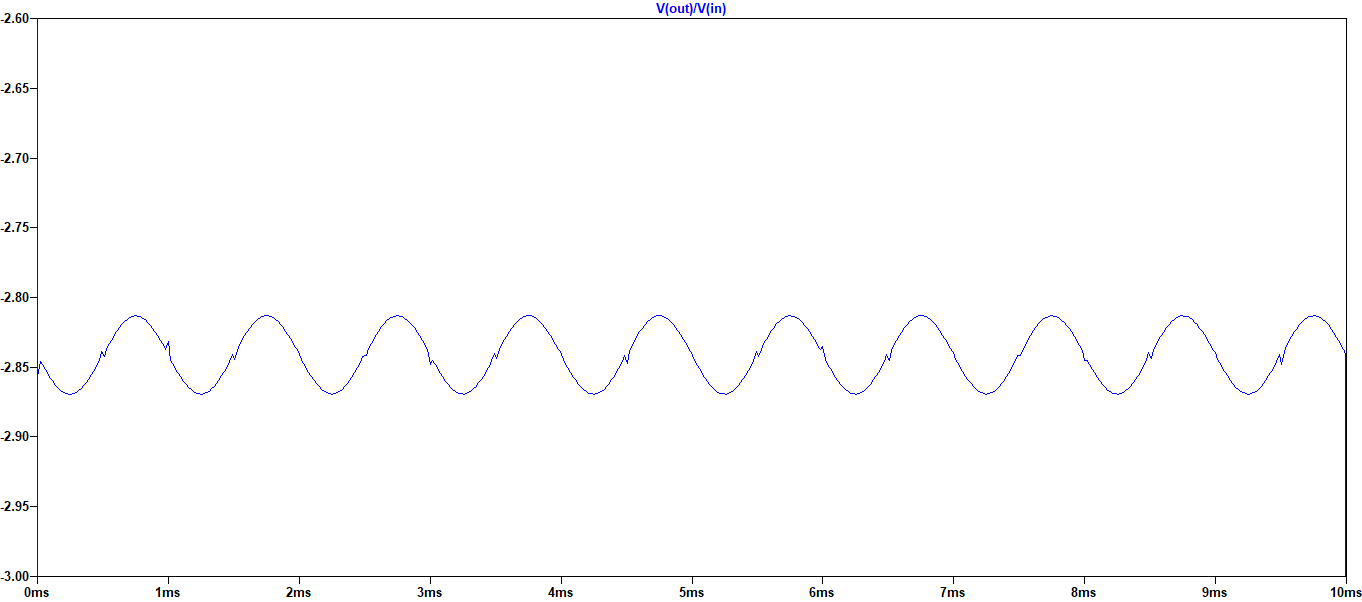
\includegraphics[width=0.7\linewidth]{es2-3-3gain.png}
  	\caption{Andamento del guadagno dell'amplificatore nei primi 10 periodi.}
  	\label{fig:gain10-3}
\end{figure}
\begin{figure}[h!]
  	\centering
 	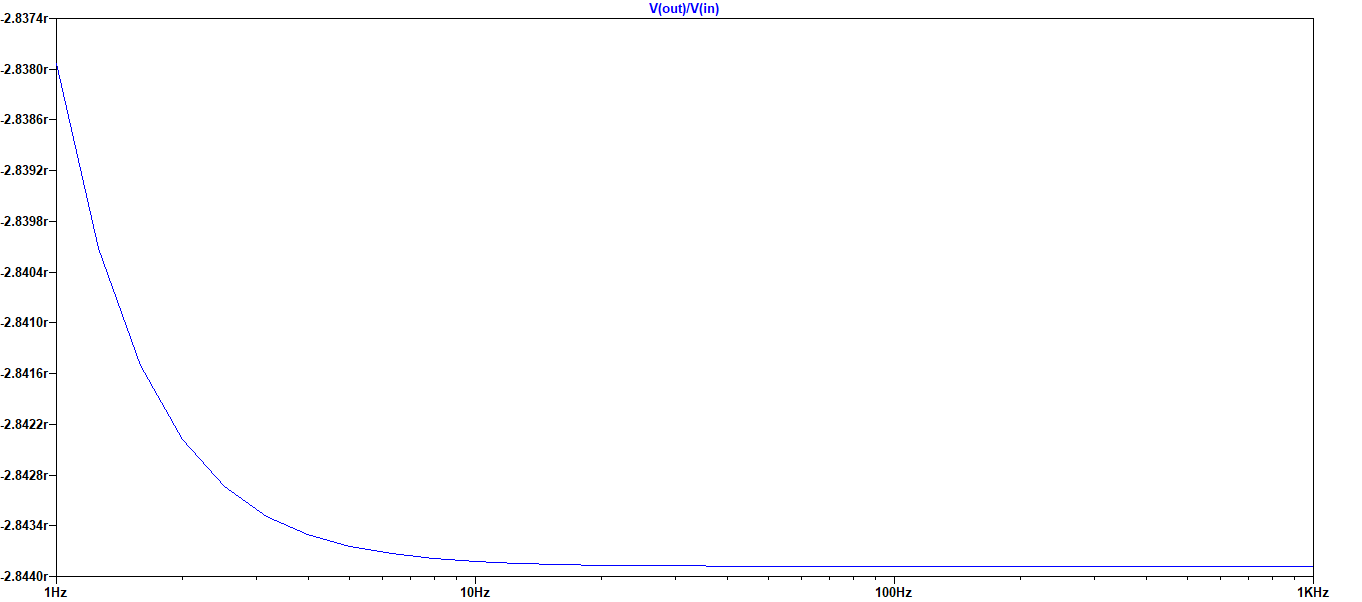
\includegraphics[width=0.7\linewidth]{es2-3-3freq.png}
  	\caption{Guadagno dell'amplificatore in funzione della frequenza del segnale di ingresso.}
  	\label{fig:gainfreq-3}
\end{figure}
I valori ritrovati in queste simulazioni coincidono con quelli trovati analiticamente. Il transitorio a basse frequenze invece e' un effetto dovuto al filtraggio attuato dai condensatori.
\newpage

\subsubsection{Verificare, solo tramite simulazioni, il massimo valore dell'ampiezza del segnale v$_I$ che garantisce una risposta lineare dell'amplificatore}
Il massimo valore dell'ampiezza del segnale in ingresso v$_I$ (trovato sperimentalmente mediante simulazioni con SPICE) che garantisce una risposta lineare da parte dell'amplificatore e' $\approx405\,mV$. Sono riportati di seguito i grafici della simulazione utilizzati dedurre questo risultato (il listato e' uguale a quello utilizzato nei punti precedenti, e' stata aggiunta solo una parametrizzazione dell'ampiezza di ingresso).
\begin{figure}[h!]
  	\centering
 	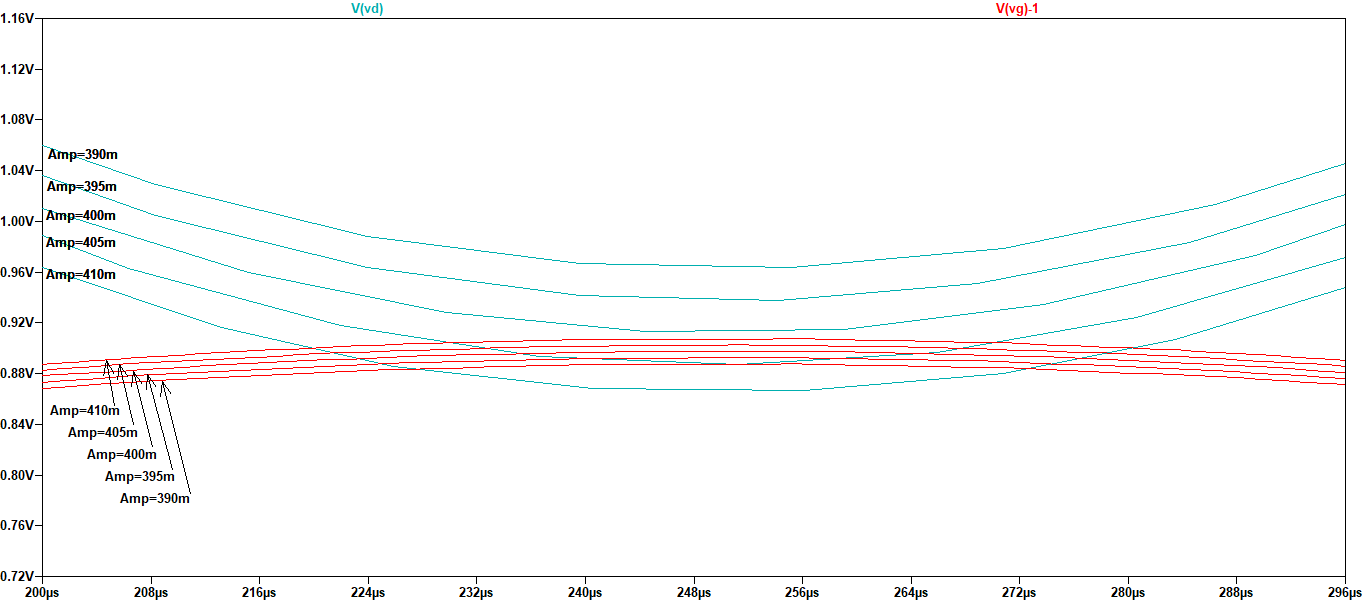
\includegraphics[width=1\linewidth]{es2-3-4waves.png}
  	\caption{Analisi sulla condizione $V_{DS}>V_{GS}-V_{tn}$.}
  	\label{fig:es41}
\end{figure}
\begin{figure}[h!]
  	\centering
 	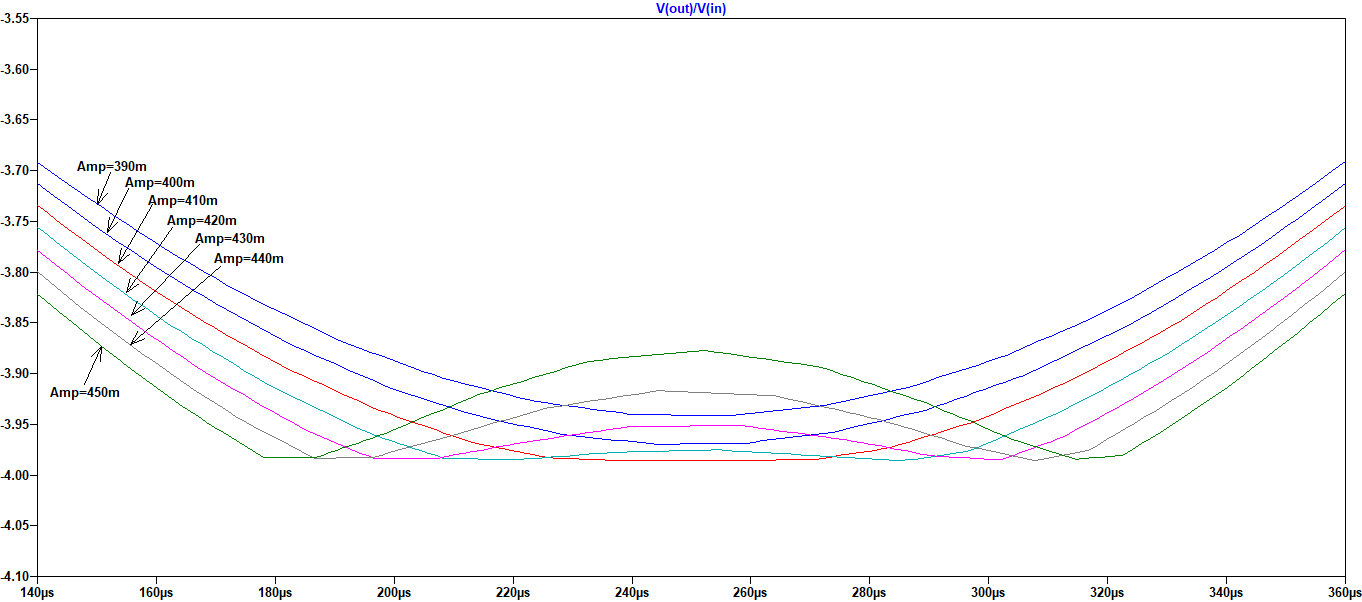
\includegraphics[width=1\linewidth]{es2-3-4gain.png}
  	\caption{Analisi del guadagno in funzione dell'ampiezza del segnale di ingresso v$_I$.}
  	\label{fig:es42-3}
\end{figure}

\newpage
\subsection{Confrontare A$_v$, R$_{in}$ e R$_{out}$ nei tre amplificatori.}
Ricapitolando, i valori di guadagno, resistenza in ingresso e in uscita dei tre amplificatori risultano essere quelli riportati in tabella (Table \ref{tabella}).\\

\begin{table}[h!]
\begin{center}
\begin{tabular}{ |c|c|c|c| } 
 \hline
   & $A_v$ & $R_{in}$ & $R_{out}$ \\ 
  \hline
 Amplificatore 1 & $-13.33$ & $ 72\,961\,\Omega$ & $87.69\,\Omega  $ \\ 
 Amplificatore 2 & $-11.068$ & $  82\,586\,\Omega$ & $ 89.87\,\Omega $ \\ 
 Amplificatore 3 & $-2.843$ & $ 2.211\,M\Omega $ & $ 2472\,\Omega $\\ 
 \hline
\end{tabular}
 \caption{Riassunto caratteristiche amplificatori.}
\label{tabella}
\end{center}
\end{table}
Notiamo che, essendo tutti e tre generatori a source comune, hanno guadagno negativo (il segnale in uscita e' in opposizione di fase rispetto a quello in ingresso). \\\\
Possiamo osservare come l'aggiunta della resistenza R$_{G2}$ nell'amplificatore 2 abbia aumentato la stabilita' dell'amplificatore (in grado di mantenere una risposta lineare per ingressi di ampiezza maggiore rispetto al primo) ma ne abbia allo stesso tempo diminuito leggermente il guadagno e aumentato resistenza di ingresso e uscita. Entrambi i primi due amplificatori hanno resistenze di uscita basse (fattore positivo) ma resistenze in ingresso non troppo elevate (fattore negativo) \\\\
Infine, osserviamo che il terzo amplificatore ha un valore del guadagno marcatamente piu' basso rispetto ai primi due, compensando pero' questa mancanza con una resistenza di ingresso molto alta (positivo per un amplificatore di tensione) e una maggior stabilita' rispetto all'ampiezza dell'ingresso. La resistenza in uscita e' tuttavia piu' alta rispetto ai primi due amplificatori (fattore negativo).

\end{document}